
\section{Alternatives}
\label{sec:Alt}

So far we have followed the main highway of string cosmology, taking as a guideline the most standard and successful approach to the early universe, namely the inflationary universe. But, even this is limited in scope. String theory's standing as the prime candidate for a fundamental theory of Nature implies that
at some point it should be able to address the earliest moments of the Universe and the questions of what happened before inflation. 
Even more interestingly, it may give rise to totally different scenarios of the early universe which manifest an intrinsic stringy structure of matter and 
provide alternatives to the inflationary scenario. 

Over the years, several attempts have been proposed to explore this important possibility. It is essentially impossible to give a full review of 
all these proposals and we content ourselves with providing a short overview of the main ideas put forward in each case, 
referring to other reviews where these ideas are discussed in more detail \cite{Gasperini:2002bn,Lehners:2008vx,Brandenberger:2008nx,Battefeld:2005av,Brandenberger:2016vhg,McFadden:2009fg,Nastase:2019rsn}. 
In particular, we follow closely the summary presented in \cite{Quevedo:2002xw} and update the original presentations there.

Before discussing concrete proposals, we point out general areas where string theory and cosmology ought to intersect:

\begin{enumerate}
\item {\it Big-bang singularity.} Within the current understanding of string theory it is not possible to address the earliest point in the history of the universe. It is widely believed that before reaching the spacetime singularity, even spacetime itself could become an emergent quantity where a fully-fledged non-perturbative formulation of string theory (or quantum gravity) will be needed. For
various approaches to address this question see e.g \cite{Damour:2000wm, Damour:2002et, Cornalba:2003kd, Hubeny:2004cn,Fischler:1998st,  Craps:2006yb, Berkooz:2007nm, KalyanaRama:1997xt, Englert:2007qb, Barbon:2015ria, Engelhardt:2015gta} (we will discuss
some in detail in what follows).


\item{\it Hagedorn phase.} Since the early days of string theory it has been known that there is a critical temperature known as Hagedorn's temperature, $T_H$. 
As the number of string states increases exponentially with energy, the partition function
\be
Z={\rm Tr} e^{-\beta H},
\ee 
with $\beta=1/T$ and $H$ the Hamiltonian, diverges at a finite temperature $T_H=\frac{1}{4\pi\sqrt{\alpha'}}$. This indicates that going back in time from the present the Universe will reach a point in which the stringy nature will dominate and at the temperature $T_H$ a phase transition may occur. The precise nature of this phase is not known but the existence of a critical temperature clearly indicates that the stringy nature of the early universe would manifest itself at finite times.
  
  \item{\it Vacuum transitions.} The work by Coleman and collaborators to address quantum tunelling transitions among de-Sitter, anti-de-Sitter and Minkowski spacetimes could mark the beginning and end of our universe in a multiverse scenario. String theory should be able to provide a proper formulation to address these questions in a full quantum theory of gravity.
  
\item{\it The wave function of the universe.} The attempts to describe a wave function of the universe and the creation of the universe from nothing, as pioneered by Vilenkin, Hartle and Hawking, were developed using a semiclassical approach to gravity. String theory, being a UV complete theory, should be able to provide a proper formulation of these proposals.

\end{enumerate} 

Addressing these questions is important for string theory (and also any other proposal of quantum gravity), and may or may not lead to an inflationary universe. It is important to hold these questions in mind and consider with an open mind possible alternatives to inflation, following where the science leads but also not being contrarian for its own sake.

\subsection{Time-dependent String Backgrounds}

Formulating string theory in time-dependent backgrounds remains an open question. However, we can find with more ease time-dependent backgrounds 
of the low-energy ten-dimensional field theory for the different string theories. In these solutions, the metric, dilaton and antisymmetric tensors may be time-dependent with cosmological implications. A natural question is to search for solutions in which 4-dimensions expand and the other ones are either 
static or expand much more slowly, in order to address the fact that we only observe four large dimensions.

For this, we first consider 
a low energy string effective action including the metric $g_{MN}$, 
the dilaton $\varphi$ and the NS-NS antisymmetric tensor of the bosonic and heterotic strings $B_{MN}$. In an arbitrary number of dimensions $D=d+1$
the bosonic action takes the form (in units where $l_s = 1$):
\be
\setlength\fboxsep{0.25cm}
\setlength\fboxrule{0.4pt}
\boxed{
S\ = \ \int d^{D}x\sqrt{-g}\ e^{-\varphi}\left( R + \partial_M\varphi
\partial^M\varphi -\frac{1}{12} H_{MNP} H^{MNP}+\cdots \right),
}
\ee
where  $H_3=dB_2$. 

Two simple classes of solutions can be described directly, including only the dilaton and metric time dependence with vanishing torsion $H_{MNP}=0$:
\begin{enumerate}
\item {\it Linear Dilaton}. 
In the string frame there is a general solution of $\varphi=A\,t$, with $A$ a constant, and  metric $g_{MN}=\eta_{MN}$ \cite{Myers:1987fv,Antoniadis:1988vi}. Going to the Einstein frame, the solutions allow for a cosmological interpretation with
metric $ds_D^2=-dt^2+t^2 dx_{\small D-1}^2$ which may be given a cosmological interpretation with linearly expanding dimensions.
\item{\it Rolling toroidal radii}. 
A simple solution with vanishing curvature is to assume that all the spatial dimensions are tori with time-dependent radii $R_i(t)$ \cite{Mueller:1989in}. For the critical dimension, in the string frame:
\be
\setlength\fboxsep{0.25cm}
\setlength\fboxrule{0.4pt}
\boxed{
R_i(t)\propto  t^{p_i}\qquad e^{-\varphi(t)}\propto  t^p, \qquad \sum_i p_i^2=1, \qquad \sum_i p_i=p.
\label{muellers}
}
\ee
For different values of the constants $p_i$, this can generate either expanding or static solutions, but without any preference for the physical case $p_i>0, i=1,2,3$ and $p_i=0$ for $i>3$. The solution in Eq. (\ref{muellers}) is recognisable as a generalised Kasner solution, extended to include a rolling dilaton.
\end{enumerate}
Even though these are not realistic cosmological solutions, they were the first steps in the study of time-dependent solutions of string theory. Over the years further solutions have been studied with interesting cosmological interpretations.\footnote{It is important to keep in mind that four dimensional cosmology experienced by observers can be an effective one, as is clearly exhibited in  mirage cosmology
\cite{Kehagias:1999vr}}
 We will discuss some of them later on. In particular, solutions generalising the original chaotic solutions of 4D gravity from Belinsky, Lifshitz and Kalathnikov \cite{Belinsky:1970ew,Belinsky:1982pk}  have been much studied with interesting mathematical structure \cite{Damour:2000wm,Damour:2002et,Belinski:2017fas}. For a recent discussion of general classes of cosmological solutions see \cite{Hohm:2019jgu,Russo:2022pgo}. An interesting concrete study of  cosmological string theory backgrounds in two dimensions for which  three and four point functions can be explicitly computed has recently been done in \cite{Rodriguez:2023kkl}.

\subsection{String/Brane Gas Cosmology}

One of the first approaches to string cosmology  was the Brandenberger-Vafa scenario \cite{Brandenberger:1988aj} (see also \cite{Tseytlin:1991xk}, for reviews and recent discussions see \cite{Battefeld:2005av,Brandenberger:2006vv}). The idea is based on the simplest manifestation of T-duality in toroidal compactifications with radius $R$:
\be
\setlength\fboxsep{0.25cm}
\setlength\fboxrule{0.4pt}
\boxed{
M^2\ = \  \frac{n^2}{4R^2} + m^2 R^2 + N_L + N_R -2\,,
}
\ee
in units of the inverse string tension $\alpha'=1/2$. The integers $n$ and
 $m$ give the quantised momentum in the 
circle and the winding number of the string in the circle, $N_{L,R}$ are the 
left and right oscillator numbers respectively. 
We can easily see that the spectrum is invariant under the simultaneous exchange of $R\leftrightarrow 1/(2R)$
and winding and momentum modes, $n\leftrightarrow m$, with a self-dual radius of $R_c=1/\sqrt{2}$. This is  the simplest manifestation of $T$-duality in string theory.

Brandenberger and Vafa explored the possible implications of this duality in cosmology and made a few interesting remarks:

\begin{itemize}
\item
The concept of distance is different for radii greater and smaller than the self-dual radius $R_c$. For radii greater than $R_c$, distance can be defined in the standard way as the dual of the conjugate momenta. But below the critical radius, the winding models play the role of momenta and it is the conjugate dual of the winding modes that properly define distance,
Supposing this duality to hold in general, it is then possible to avoid distances smaller than the self-dual radius as the physics at those distances is equivalent to the physics at distances greater than the self-dual radius. In this sense, this concept of minimal length offers a way to avoid the big-bang singularity.
\item
Winding modes, and the tension associated to them, suggest that energetics can favour a small value of the corresponding circles. If winding modes annihilate with modes of the opposite winding, the corresponding circle can grow as large as possible and so essentially de-compactify. $p$-dimensional objects generically intersect in at most $2p+1$ dimensions. Therefore, winding strings ($p=1$) can annihilate in three spatial dimensions and allow these dimensions to become large, offering a potential explanation of the fact that we live in $3+1$ dimensions. This proposal is one of the very few concrete proposals to explain one of the most clear experimental properties of our observed universe, namely that it has three large dimensions and that the other ones, if they exist, are somehow hidden to us.\footnote{As mentioned in the brane inflation section, there are other proposals to address the dimensionality of spacetime \cite{Burgess:2001fx,Karch:2005yz, Durrer:2005nz}. For an independent  early proposal see \cite{Gibbons:1986uu}. } Some numerical studies have been made of this proposal, with mixed results (see for instance \cite{Sakellariadou:1995vk,Greene:2009gp,Greene:2012sa}).

\item
Independent of the dimensionality issue, this proposal emphasises that the current approach to cosmology in the FLRW model should be expanded such that the stress-energy tensor contribution to the density and pressure of the universe  should be that of a gas of strings and branes entering into the Einstein's equations used to study early universe cosmology. Extrapolating back in time from the present we reach higher and higher temperatures and at the critical Hagedorn temperature $T_H$ there is an expected  phase transition to a new phase dominated by a gas of  strings and branes \cite{Battefeld:2005av,Brandenberger:2006vv, Alexander:2000xv, Easther:2002qk, Easther:2003dd}. This is 
illustrated in figure \ref{Hagedorn}. Even though the nature of this phase is not known its cosmological implications may be possible to explore. 
\end{itemize}

\begin{figure}[t]
\begin{center}
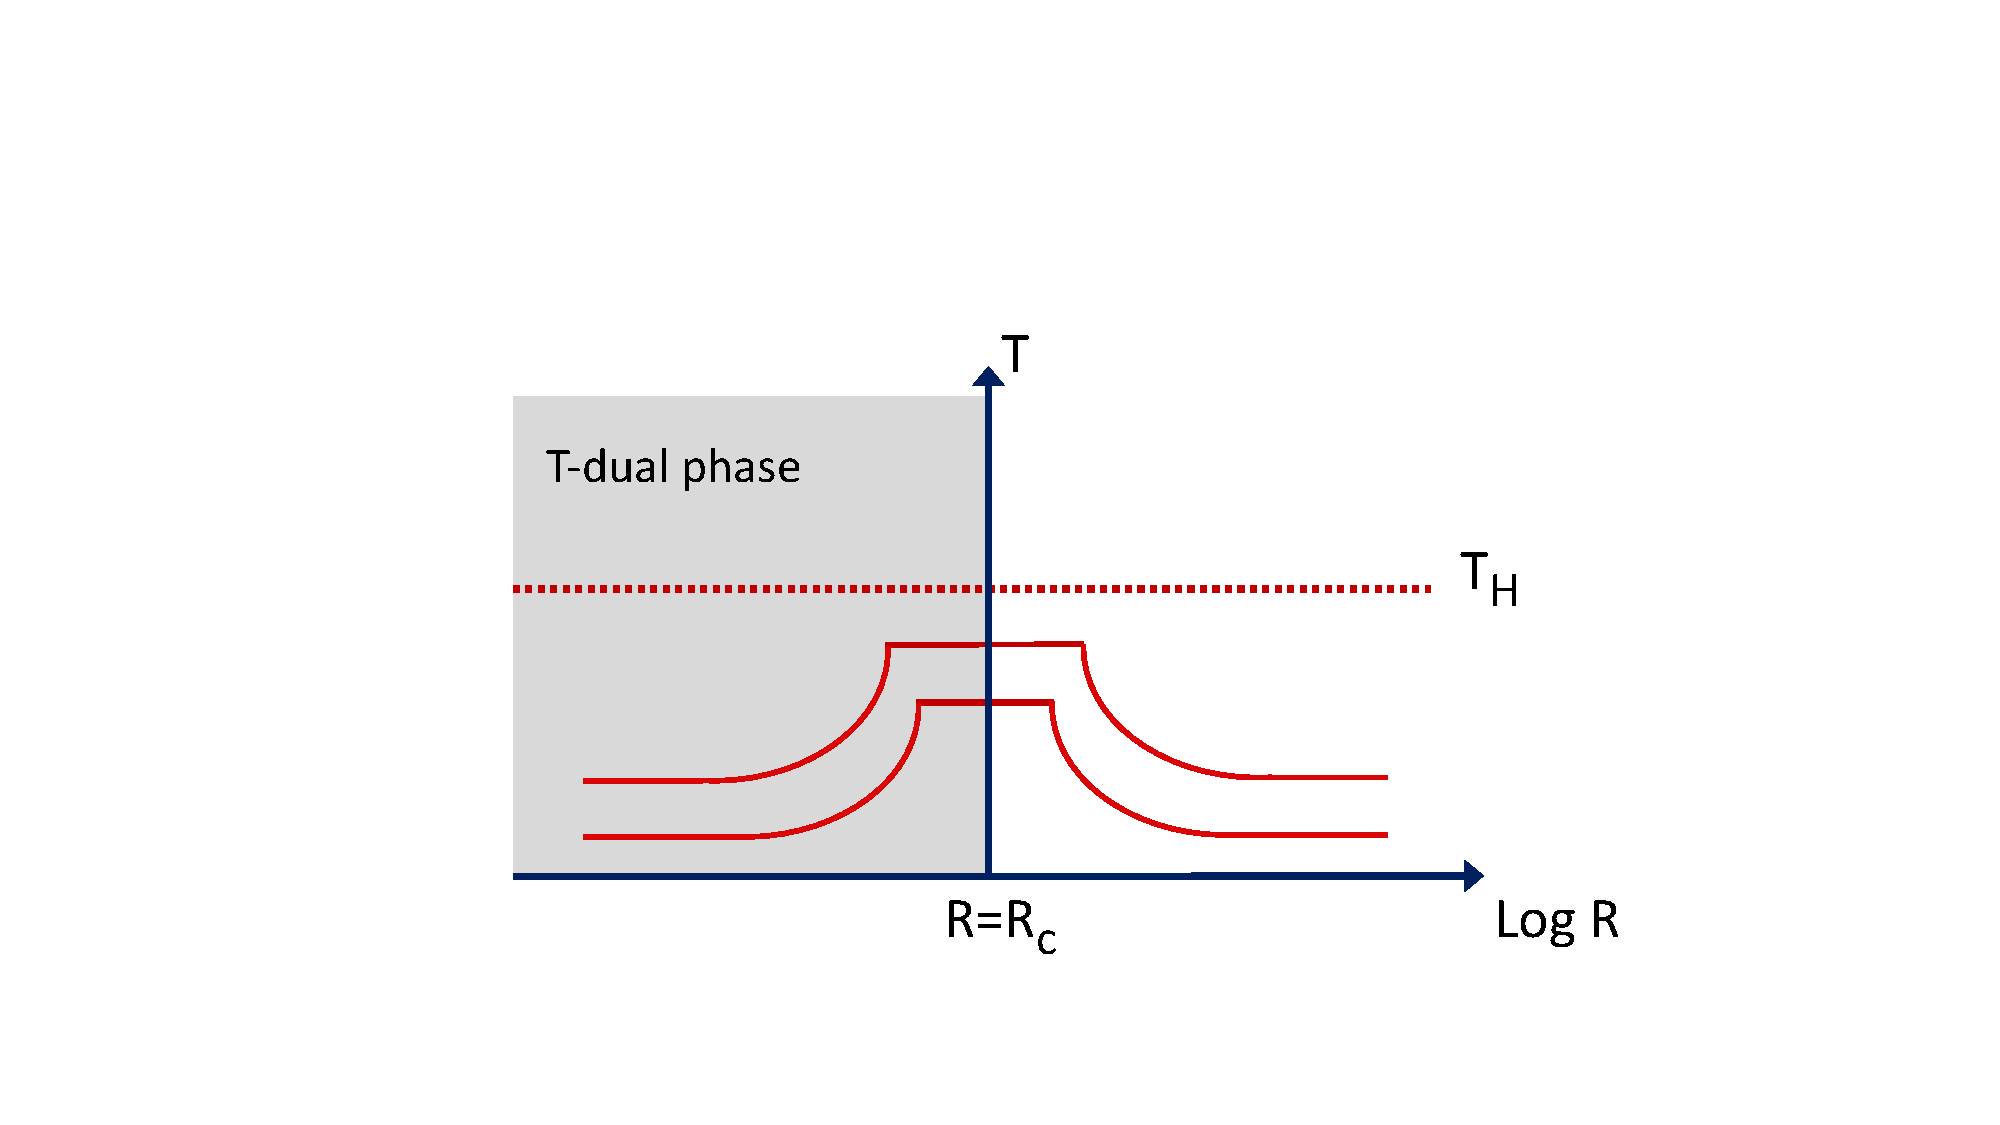
\includegraphics[width=170mm,height=90mm]{Sections/Figures/Hagedorn.pdf} 
 \vskip -25pt
\caption{Temperature $T$ against the radius of the extra dimensions $R$ in string gas cosmology illustrating the Hagedorn temperature as a limiting temperature in string theory and the two dual phases of T-duality separated at the self dual point $R_c$.} \label{Hagedorn} 
\end{center}
\end{figure}

Although these ideas are very attractive, they have been mostly formulated in  simplistic cases for which all of the dimensions are circles. They have not been formulated on realistic set-ups in which chiral matter like in the Standard Model is present. A further issue is that the intuition that strings under tension causes cycles to shrink only holds under the assumption that the dilaton has been stabilised, e.g. by some standard mechanism such as gaugino condensation. This is manifest in 4-dimensional Einstein frame, where the radion is a linear combination of the string frame dilaton and radion.

The lack of understanding of the Hagedorn phase is also a major obstacle at the moment. However, these ideas may eventually be applicable in more realistic frameworks and it is worth to keep them in mind. In particular, after the emergence of the brane-world scenario, generalisation of these ideas may add to the arguments for the critical dimensionality of spacetime. For example, for D4 branes ($p=4$) to avoid annihilating each other they need to live in a universe with dimension greater than $2p+1=9$. This may put a bound on the brane dimensionality to be smaller than four \cite{Burgess:2001fx,Durrer:2005nz}.  A more detailed study for IIB string theory singles out  D3 and D7 branes \cite{Karch:2005yz} which are precisely the branes which host the Standard Model in F-theory and other local D-brane constructions of the Standard Model. For a realisation of inflation making use of the Hagedorn phase see \cite{Abel:2003jh}.

In the regimes where effective field theories are applicable, there also remains the standard challenge of implementing the scenario in realistic set-ups including moduli stabilisation (for a study of a possible realisation in type IIB string theory, see \cite{Frey:2005jk}).

\subsection{Pre Big-Bang Cosmology}

In the 1990s Veneziano and collaborators went beyond the  Brandenberger-Vafa  proposal by considering the possibility of
 $T$ duality in cosmological backgrounds much closer to  the FRW type. For an ansatz  of the type:
$ds^2= -dt^2 + \sum_{i=1}^d a_i^2(t)\ dx_i^2$
it can be seen that $T$ duality is a symmetry of the 
equations of motion acting as:
\be
\setlength\fboxsep{0.25cm}
\setlength\fboxrule{0.4pt}
\boxed{
a_i(t)\rightarrow \frac{1}{a_i(t)},
 \qquad \varphi\rightarrow \varphi - 2 \sum_i\log a_i.
 }
\ee
Since $a_i(t)$ represent the scale factor, as in FRW, this 
has been named {\it scale factor duality} \cite{Veneziano:1991ek}. Thus we can see that expanding and
contracting universes are related by this symmetry.

Gasperini and Veneziano combined this  symmetry with the standard time-reversal symmetry:
$a(t)\leftrightarrow a(-t)$, to allow for a possibility of considering cosmology before  $t=0$, in which the Hubble parameter increases instead of decreases.
Without duality, the symmetry under $t\rightarrow -t$ would send
$H(t)\rightarrow -H(-t)$ but, combining
 this with scale factor duality, it provides four different sign 
combinations for $ H(t)$. 
If the universe at late times is decelerating, $H$ would be a decreasing
 monotonic function of time for `positive' $t$, but a combination of duality
 and the 
$t\rightarrow -t$ transformation can give rise to  $H(-t) = H(t)$ so 
that this
 function can be even, as shown in figure \ref{PreBigBang}. They therefore proposed a scenario in which the universe accelerates from negative times
 towards the big-bang and then decelerates after the big-bang. The 
acceleration would 
indicate a period of inflation before the big-bang without the need of an
 scalar
 potential. This scenario is called {\it Pre Big-Bang Cosmology} \cite{Gasperini:1992em,Gasperini:2002bn,Gasperini:2007vw}, see also \cite{Tseytlin:1991wr}. 

A concrete solution for this system corresponds to the isotropic case
$a_i=a_j\equiv a(t)$ for which:
\be
a(t)= t^{1/\sqrt{d}}\qquad t>0\ , 
\ee
with a constant dilaton. For this solution, $H(t)\sim 1/t$ decreases monotonically 
with time. By applying the transformation $t\rightarrow -t$ and duality we
 can generate the four different branches of solutions:
\be
a(t)=t^{\pm1/\sqrt{d}}\qquad t>0, \qquad a(t)= \left(-t\right)^{\pm1/\sqrt{d}}\qquad t<0, \label{veneziano}
\ee
with 
$\varphi_\pm (\pm t)\ = \ (\pm\sqrt{d} - 1) \log(\pm t)$.

\begin{figure}[t]
\begin{center}
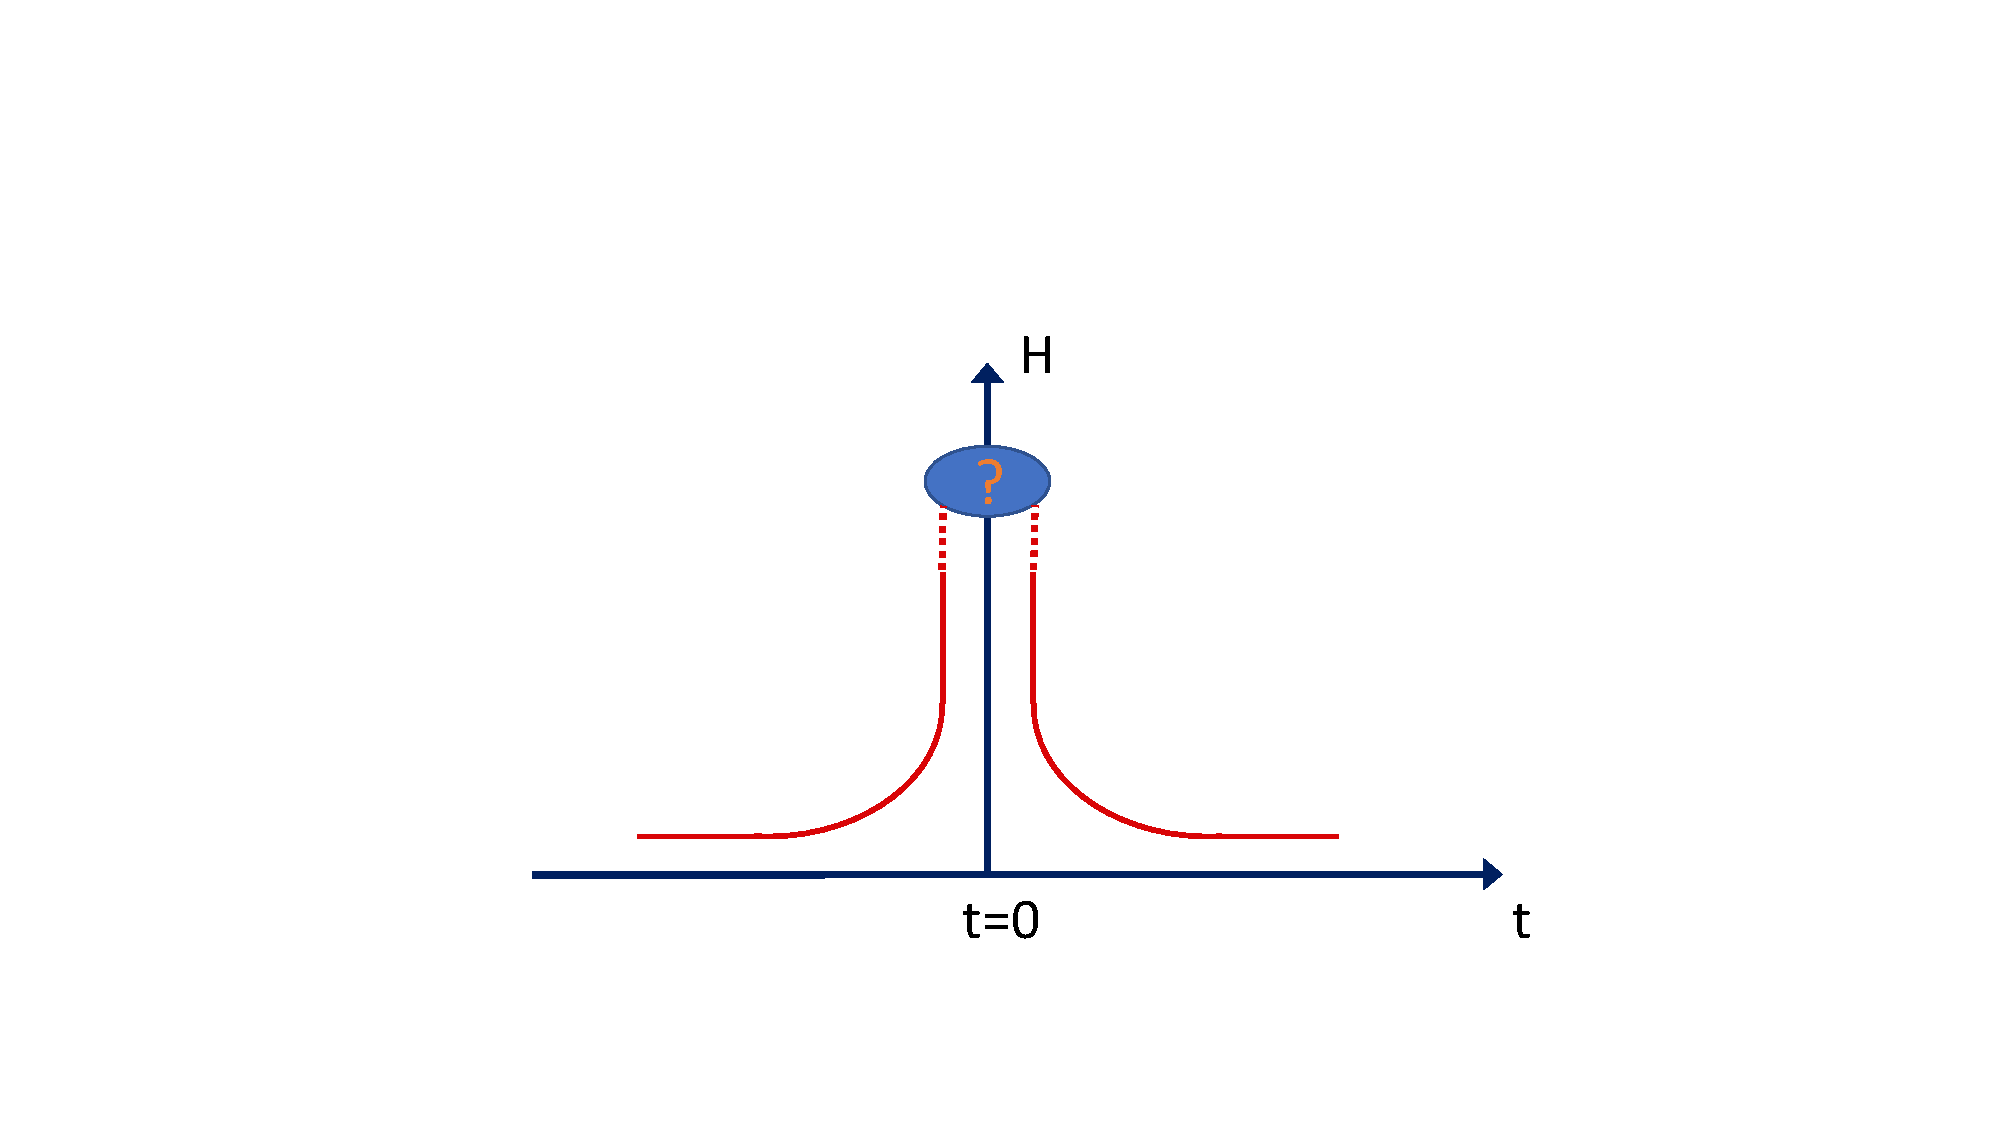
\includegraphics[width=160mm,height=70mm]{Sections/Figures/PreBigBang.pdf} 
\caption{Possible realisation of the pre big-bang scenario with the past and future regions expected to match at the singularity with strong coupling and large curvature.} \label{PreBigBang} 
\end{center}
\end{figure}

In the two branches for which  $H>0$, the universe expands, which provides an 
interesting realisation of the pre big-bang scenario, as illustrated in figure \ref{PreBigBang}.
The solutions are such that there is  a singularity at $t=0$ but also in this
 region the dilaton blows up implying strong string coupling. 
The hope is that non-perturbative string effects provide a smooth 
matching between these two branches. Since the weak 
coupling perturbative string vacuum appears as a natural initial condition 
in the pre big-bang era, the scenario consists of an empty cold
 universe in the infinite past which expands in an accelerated way 
towards a region of higher curvature. Eventually, it approaches the region of 
strong coupling and large curvature, which is assumed will match smoothly
 to the post big-bang branch in which the universe continues expanding but now with
decelerated expansion.

 The spectrum of density perturbations in this scenario has been estimated, and claimed not to contradict the recent 
observations. The scenario also
provides testable differences compared to inflation via the tensor 
perturbations, which could be put to test in future searches for gravitational waves.

While this scenario has very interesting features, it has also been subject to criticism for several reasons. First, as
 the original authors pointed out,
 the main problem to understand is the graceful exit question,
namely how to pass smoothly from the pre to post Big-Bang period. As this requires describing the big-bang singularity, this is a major challenge. 
Close to the Big-Bang the perturbative treatment of 
string theory does not hold since the dilaton and the curvature increase,
 implying strong string coupling. Therefore, there is no concrete way to
 address this issue within the framework where the theory is formulated. 
Another important
 problem is the fact that the moduli are neglected from this analysis and 
there has to be a mechanism that stabilises the extra dimensions. 
Furthermore, the scale factor duality symmetry that motivated the scenario is not
 clearly realised
in  more realistic settings with nontrivial matter content and the fact that the 
dilaton will eventually be fixed by non-perturbative effects may change the 
setting of the scenario. 

On the other hand, this represents an explicit proposal for the early universe with interesting string inputs which  may prove useful in a
more realistic scenario. Furthermore, the study of this scenario has led to interesting potential signatures from gravitational waves and has triggered
much activity in this direction. After the detection of gravitational waves and the future progress in this direction, these preliminary studies of gravitational waves
from a string theory perspective may prove very useful for experimental searches and may be a useful guideline for alternative proposals.

\subsection{Ekpyrotic/Cyclic Scenario}

The ekpyrotic scenario (illustrated in figure \ref{Fig:HW}) was developed in the early 2000s by Khoury, Ovrut, Steinhardt and Turok and has presented itself as an interesting alternative to the inflationary universe, drawing its original inspiration from string theory \cite{Khoury:2001wf,Khoury:2001bz,Steinhardt:2002ih, Lehners:2008vx}.

The proposal was first formulated within a particular string theory scenario, namely the 11-dimensional formalism of Horava and Witten with one of the dimensions compactified in an interval $I$ (understood as a $Z_2$ orbifold of a circle $I=S^1/{\bf Z}_2$). 
The endpoints of the interval correspond to two parallel 10-dimensional spaces or {\it end of the world branes}  
which are the `fixed points' of the orbifold, with each hosting $E_8$ gauge theories, providing a strong coupling version of the heterotic string.
 Further compactification on a six-dimensional Calabi-Yau manifold then leaves two 
4D worlds at the ends of the interval in the 5D bulk. In principle, quasi-realistic
 models can be obtained from this approach, mostly using the topological
 properties of Calabi-Yau manifolds. It turns out that besides the end
 of the (interval) 
world branes, which we may also refer to as boundary  branes,
 there are also five-dimensional branes in these compactifications (M-branes) that are not restricted to
live at the fixed points and can move through the bulk.
 These are called bulk branes in order to differentiate them from the boundary branes. Overall, these
 configurations are reminiscent of models with both D-branes at orbifold singularities and also mobile branes.

\begin{figure}[t]
\begin{center}
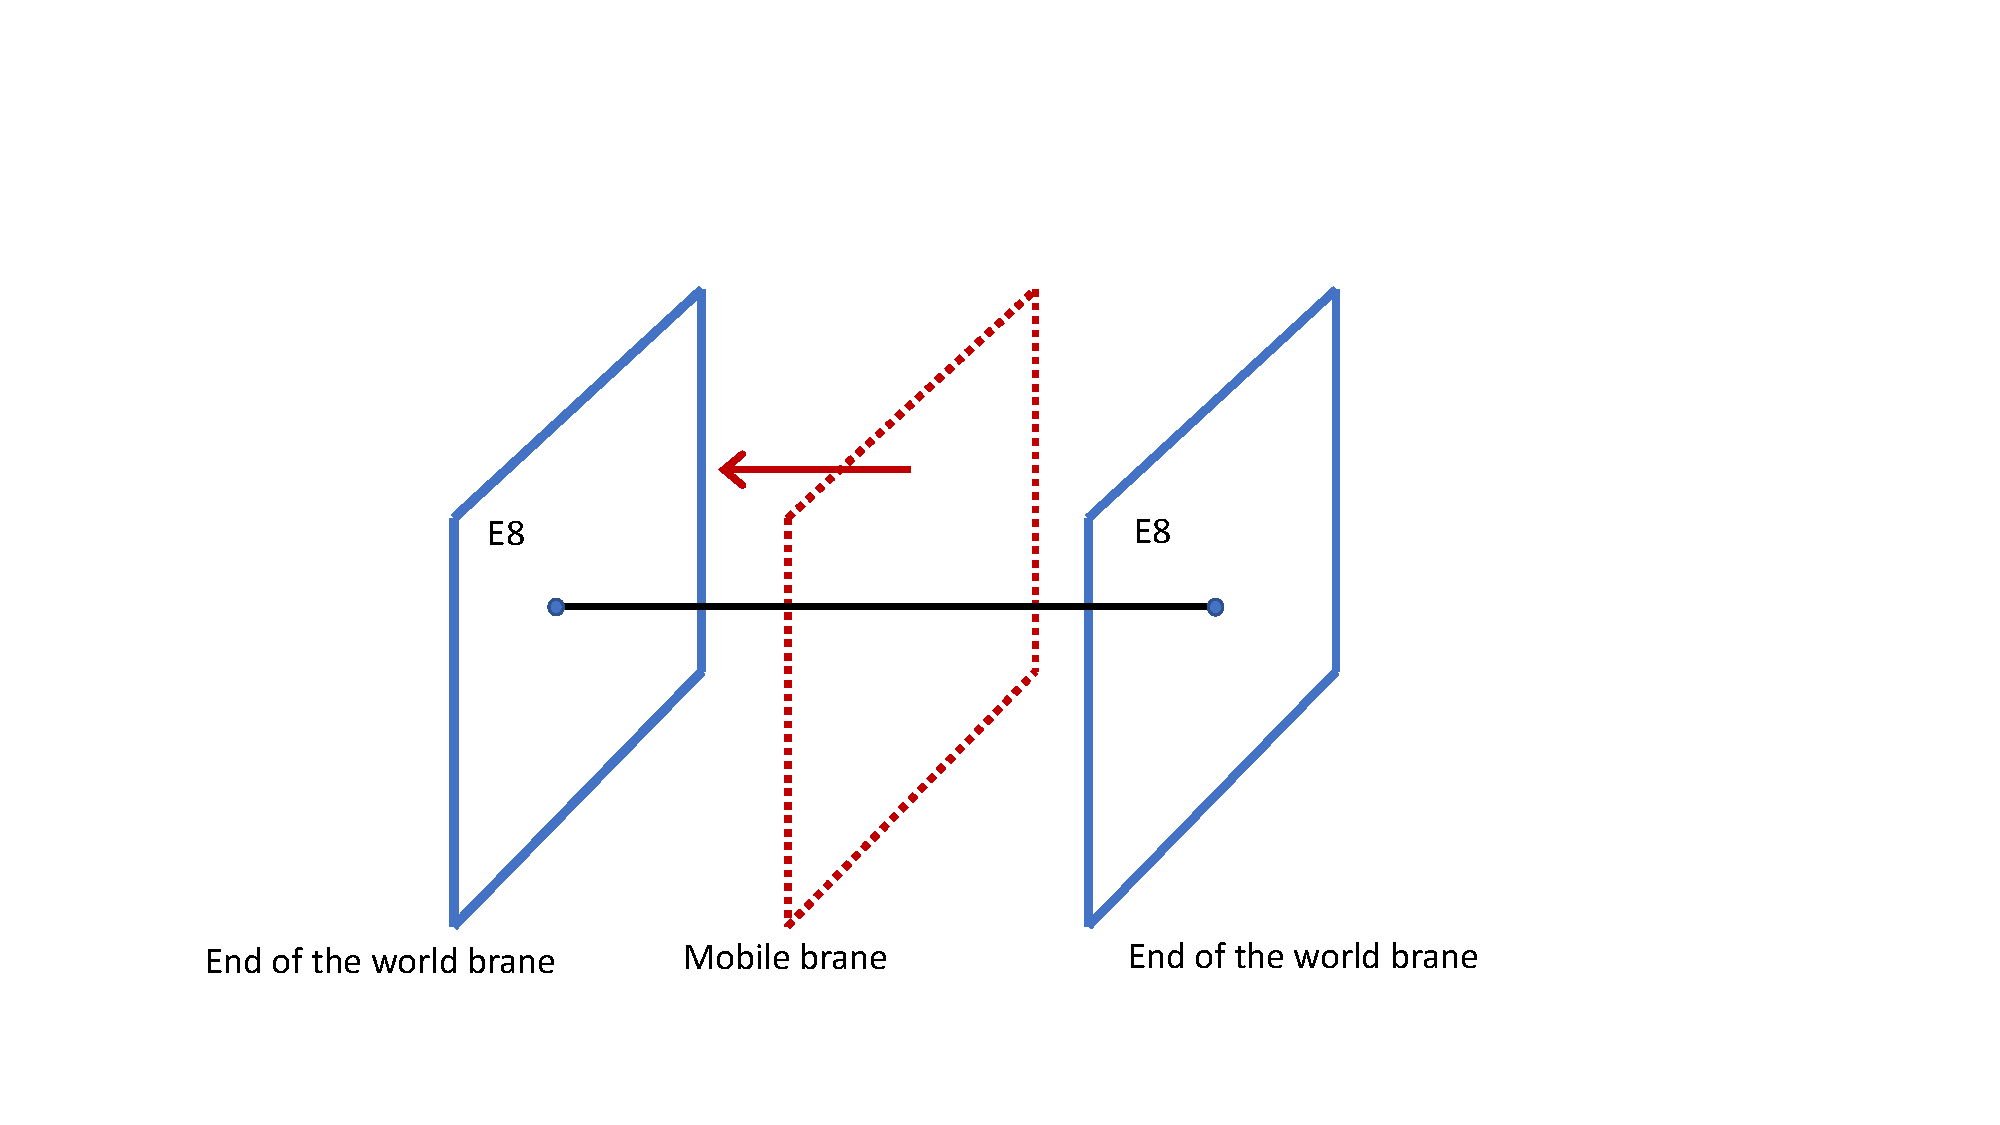
\includegraphics[width=150mm,height=90mm]{Sections/Figures/Horava.pdf} 
\caption{The Horava Witten scenario. 
Two surfaces or end of the world branes, each at the end of 
the interval, provide chiral matter and possibly interesting cosmology as proposed in the ekpyrotic/cyclic scenario. Ripples on the mobile brane may be the source of density perturbations.} \label{Fig:HW} 
\end{center}
\end{figure}

Khoury {\it et al.~} also made an interesting proposal regarding the collision of branes, not to obtain inflation as in the brane inflation discussed in section \ref{sec:infla}, but as an alternative to inflation. The original idea
was to assume that a (hidden) bulk brane going from one boundary of the interval to the other end, would collide with the second (visible) boundary 
brane and produce the Big-Bang. The bulk brane would be almost BPS -- by which it was 
meant that it is essentially parallel to the boundary branes --  and move freely and slowly from one end of the interval to the other.
Small quantum fluctuations  induce some ripples on this brane which, when colliding with the visible end of the world 
brane, would produce the density fluctuations measured in the CMB. There is 
no need of an inflation potential for this. A potential of the type 
$-e^{-\alpha Y}$, with $Y$ is the separation of the branes, was proposed, although not derived, describing  the attraction of the branes. 
The 5D metric is taken with a warp factor that implies that the
motion is
 from smaller to larger curvature across the interval and therefore the scale 
factor depends on the position of the brane in the interval. 

This proposal has received several critics The first involves 
the standard problems solved by inflation. The horizon and flatness
problems require the  branes to be almost exactly parallel before collision,
which may require a fine-tuning of initial conditions. Although relics such as
monopoles will not be present if the collision temperature is low
enough this argument needs to be properly quantified. There is also no general natural
dilution, as in the exponential expansion of inflation, making the solutions of these problems more
difficult in general.  The issue of fine tuning of
 the initial conditions in the ekpyrotic scenario has been widely debated.

However, the most prominent difficulty of this scenario is the following:
in a 4D description, $\dot a<0$ before the collision, while it is expected that $\dot a>0$ after the collision,
 which requires a transition from contraction to expansion, without, in principle, crossing a 
singularity. This is a problem because it violates the null energy condition.

Let us briefly review this argument. Consider gravity coupled to a scalar field: (setting $\kappa_5=1$) 
\be
{\cal L}\ = \ \sqrt{-g}\left( R-\frac{1}{2} 
\partial_\mu\phi\partial^\mu\phi-V(\phi)\right),
\ee
The energy density and pressure are given by:
\be
\rho\ = \ \frac{1}{2}\dot\phi^2 + V, \, \qquad p\ = \ \frac{1}{2}\dot\phi^2 - V .
\ee
Therefore, Einstein's equations imply:
\be
\setlength\fboxsep{0.25cm}
\setlength\fboxrule{0.4pt}
\boxed{
\dot H =  -\frac{1}{2}\left(\rho+p\right) = 
-\frac{1}{2}\dot\phi^2 \leq \ 0.
}
\ee
This implies that $H$ is  monotonically decreasing and 
we cannot go from contraction ($H<0$) to expansion ($H>0$).

This problem motivated a second version of this scenario 
 which does not include the mobile brane but considers the collision of the two end-of-the-world branes. In this case, there is 
a singularity at the moment of collision, since the size of the fifth dimension reduces to zero, 
 which, in principle, could allow a transition from 
contraction to expansion. The singularity happens only in the extra dimension because the scale 
factors of the branes remain finite during the process. After the collision, the two branes separate again and the scale factor increases (see Fig. \ref{F:ekpyvar}).
\begin{figure}[t]
\begin{center}
\vskip -10pt
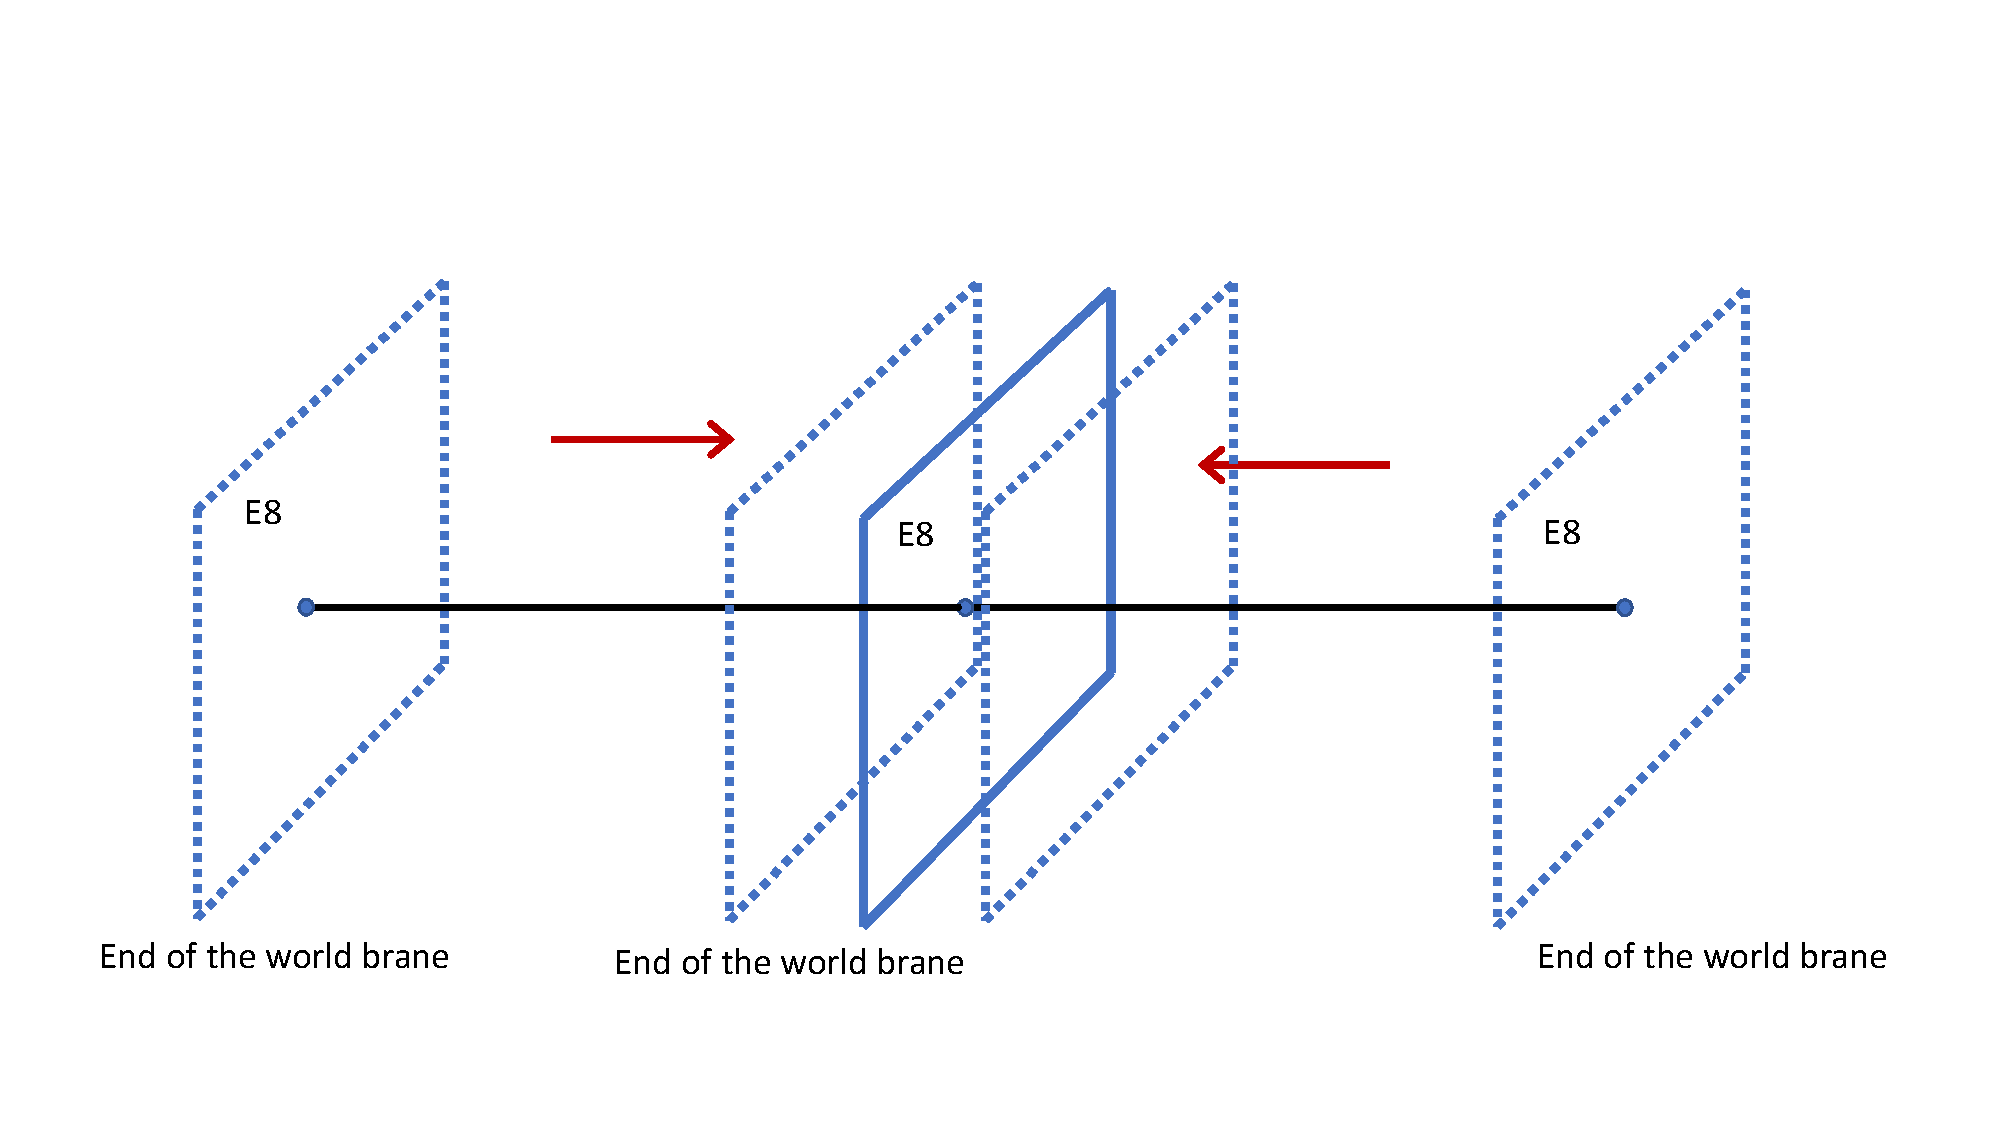
\includegraphics[width=140mm,height=90mm]{Sections/Figures/Cyclic.pdf} 
\caption{A variation of the original ekpyrotic universe scenario in which the end-of-the world branes approach each other, pass through their overlap point and at some point return, so completing the cycle.} \label{F:ekpyvar}
\end{center}
\end{figure}

In terms of a four-dimensional EFT,  this process can be understood in similar terms to the discussion of the
 Pre Big-Bang proposal. Neglecting the scalar potential and identifying  the separation between the branes with 
 the string dilaton (as it happens in the Horava-Witten scenario) we can use equations (\ref{veneziano})
for the case $d=4$. Out of the four possibilities provided by the choices of sign we can choose:
\be
a(t)\ = \ |t|^{1/2}, \qquad \phi\ = \ \phi_0\pm \sqrt{3}\log|t|.
\ee
The  scale factor $a(t)$ goes from contraction
at negative $t$  to expansion at positive $t$. This still leaves the choice of sign for the 
dilaton open. Since the string coupling is proportional to 
$e^{-\phi}$, the negative sign  choice that was taken in the pre big-bang scenario
corresponds to strong string coupling whereas the positive choice, 
chosen in the ekpyrotic scenario, implies weak coupling at $t=0$. Therefore 
Khoury and collaborators conjectured that the transition is smooth at the singular point and  afterwards the branes may start to separate again. 



This leads us to a third version of this scenario that corresponds
 to the {\it cyclic universe} \cite{Steinhardt:2002ih}. In this case, the two branes keep separating and
 passing through each other an infinite number of 
times, as long as the interacting 
potential has a very particular form. For instance, for a potential like that of
 Fig. \ref{Fig:cyclic}, we may describe the universe's history by starting on the right
 hand side corresponding to the current time. The potential is taken to be slightly positive 
and with a slightly negative slope, reflecting the fact that the universe accelerates today as in quintessence.

 Since the slope of the potential is  negative, the scalar field
will start rolling towards smaller values representing the higher dimensional picture of the branes approaching each other.
At some point the field will cross the $V=0$ point and its energy density
 will mostly be kinetic. The potential rapidly becomes negative
 and then the energy density $\rho= V+\frac{1}{2}\dot\phi^2$ touches zero, implying 
that the universe starts contracting. Since the kinetic energy is also 
large, the 
field  passes through the minimum, towards the flat region at infinite
$\phi$ or zero string coupling, where the branes collide
and bounce back with enough energy to re-cross the steep minimum and
go to the right hand side of the 
potential, where it returns to a radiation dominated era,before repeating the
whole cycle again.
\begin{figure}[t]
\begin{center}
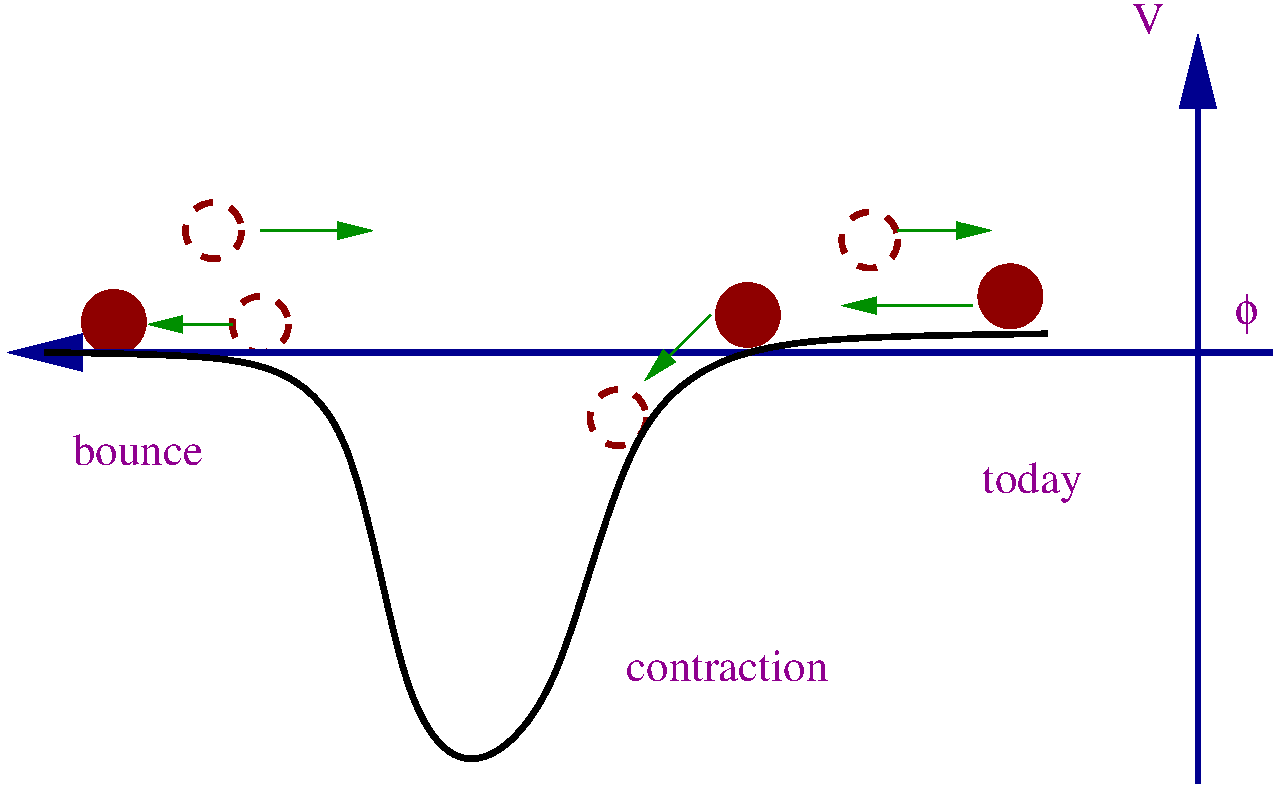
\includegraphics[width=100mm,height=60mm]{Sections/Figures/cyclic2.pdf} 
\caption{An illustration of the potential and
 trajectory of the field in the cyclic universe. Figure taken from  \cite{Quevedo:2002xw}. } \label{Fig:cyclic} 
\end{center}
\end{figure}

The different versions of this scenario claim to resolve the same questions addressed by inflation. 
For instance, the claim is that the horizon problem does not exist if there is a bounce, since there will be
 clear causal contact between different points. In the cyclic version,
the late period of mild inflation plays a similar role as the
original inflationary scenario by dissolving unwanted objects such as 
like magnetic monopoles, and emptying the universe for the next cycle, thereby also solving the
flatness problem.
 Furthermore, the spectrum of perturbations has been claimed to be 
consistent with observations. Although this issue has been debated, 
all parties seem to agree that the methods used so far are not entirely
conclusive one way or another.

There are some  interesting aspects to these proposals, 
especially regarding  the revival of the cyclic universe. A cyclic universe was originally proposed in the 1930's 
but it was immediately realised that the entropy increases on each cycle, requiring the length of
each cycle to increase. Extrapolating back in time, we reach 
an initial singularity rendering the model only semi-eternal,
similar to eternal inflation which also requires a beginning. So it is not really cyclic.

In the current version, the old entropy problem is claimed to be solved as follows. Although it is true that the total entropy 
 increases with each cycle, the entropy of matter is always the same 
at the end of each cycle. This is due to the present accelerated expansion
 which dilutes matter and so renders the universe essentially
 empty, actually one particle per Hubble radius, before restarting the cycle.
This scenario was found in the context of the ekpyrotic scenario,
but it is clearly independent of it and may have other  realisations.

Another interesting point of this scenario is that it connects the early
 universe and 
late universe in a coherent way. The current acceleration is used as a way 
 to prepare the universe to the next cycle.

 
Even though the scenarios were motivated in terms of string theory, the 
kind of scalar potentials that are needed for this scenario to work are relatively contrived and have not been 
derived from the underlying theory.
 This is certainly an important  question to be addressed before these models 
can be considered genuine string/M-theory models. In this sense, these scenarios are 
 presently at a similar stage as D-brane inflation was in 1998 where the scalar 
potential was only guessed, rather than explicitly calculated as in the 
brane/antibrane \cite{Burgess:2001fx, Kachru:2003sx}. 
Finding a potential with the 
proposed properties represents a clear open challenge for these models.
 
From a string theory perspective, there are several other problems with this scenario. 
In particular, the assumption that 
the moduli of the Calabi-Yau manifold are fixed and decoupled is not justified.
 Nonetheless, the main problem to deal with remains the big-bang singularity 
giving rise to the bounce. This is a strong assumption as description of the bounce relies on strong coupling and non-perturbative dynamics.
For further developments regarding the implementation of the ekpyrotic scenario see \cite{Buchbinder:2007ad}. For a comprehensive review of the subject see \cite{Lehners:2008vx}.


\medskip
In summary, what the three scenarios: of pre big-bang cosmology, string/brane gas cosmology and ekpyrotic/cyclic have in common is that they
contemplate a period of contraction, and represent examples of bouncing cosmologies.
For a nice recent review on such bouncing cosmologies, see \cite{Brandenberger:2016vhg}.

\subsection{The Rolling Tachyon}

As we have seen in section \ref{sec:infla} the open string tachyon plays an important role in brane anti-brane inflation. It provides the natural way to end inflation and is the source of production of lower dimensional branes like stringy cosmic strings.

From the formal perspective, there has been concrete progress in understanding from first principles the physics of the open string tachyon. In particular, using string field theory Sen managed to extract substantial information regarding the tachyon potential \cite{Sen:2002nu} (for a review see \cite{Sen:2004nf}). This is actually one of the only cases in which a scalar potential has been derived directly from string theory. It is therefore worth exploring the potential cosmological implications of the tachyon field, independent of brane inflation.
 
String calculations suggest that to all orders in derivative expansion these actions take a Born-Infeld form.
\be
\setlength\fboxsep{0.25cm}
\setlength\fboxrule{0.4pt}
\boxed{
{\cal L}\ = -\ V(T)\ \sqrt{1- g^{\mu\nu} \partial_\mu T \partial_\nu T}\ ,
}
\ee
where $V(T)$ can take different forms depending on the type of string theory, 
namely bosonic or supersymmetric. 

First, Sen studied the rolling of the tachyon to its asymptotic minimum 
$T\rightarrow \infty$ and concluded that, even though the vacuum should correspond to the closed string vacuum and the unstable D-brane system 
(such as brane/antibrane pairs or non BPS D-branes) has decayed, the energy density is still localised. Furthermore, 
he was able to prove that the resulting gas corresponds to a pressure-less gas. This is easy to see from the
effective action above for which the stress energy tensor
for a time-dependent tachyon implies
\be
\rho\ =\ \frac{V(t)}{\sqrt{1-\dot T^2}}\ , \qquad p\ =\ -V(T)\sqrt{1-\dot T^2}
\ .
\ee
 For constant energy density, the pressure behaves as $p=-V^2/\rho$ and at the
 minimum in $T\rightarrow \infty$ we know that $V\rightarrow 0$ and so 
$p\rightarrow 0$. The equation of state is $p= \omega\,\rho$ with $\omega=-(1-\dot T^2)$ and therefore
$-1\leq \omega\leq 0$.

For a time-dependent tachyon field, we should actually consider a time-dependent metric such as the one of  FLRW. 
In \cite{Gibbons:2002md} this was done, obtaining the 
Friedmann's equations for this Lagrangian coupled to 4D gravity:
\begin{subequations}
\begin{empheq}[box=\widefbox]{align}
H^2 & =  \frac{8\pi G}{3} \frac{V(T)}{\sqrt{1-\dot T^2}} - \frac{k}{a^2}\ , 
\nonumber \\
\frac{\ddot a}{a} & =   \frac{8\pi G}{3} \frac{V(T)}{\sqrt{1-\dot T^2}}
\left(1-\frac{3}{2} \dot T^2\right)\ .
\end{empheq}
\end{subequations}
Even without actually solving these equations, it can be easily seen that the
energy density decreases with time, while $T$ increases relaxing towards the
 asymptotic minimum of the potential. In the meantime the universe expands,
first accelerating ($|\dot T|<2/3$) and then decelerating ($|\dot T|>2/3$).
Depending on the value of the spatial curvature
 $k=0,1,-1$, the scale factor $a(t)$ goes to a constant for $k=0$, 
to a Milne universe $a(t)\rightarrow t $ for $k=-1$ or re-collapses, for 
$k=1$.

Another natural question is whether
this tachyonic potential can give rise to
 inflation by itself. However, this is challenging
The main reason is the absence of small parameters in the potential 
that can be tuned to give a sufficiently slow roll. See however \cite{Padmanabhan:2002cp,Frolov:2002rr,Fairbairn:2002yp,Cremades:2005ir}.

As well as open string tachyons, string spectra can also include tachyons in the closed string spectrum.
The situation with closed string tachyons is more complicated and less understood. One way to 
see this is that, while the open string tachyon triggers the disappearance of D-branes after their collision 
by settling to the minimum of the potential, closed string tachyons are intrinsically gravitational and so their condensation 
may represent the disappearance of spacetime itself. Some simplifying configurations have been studied in which this happens for localised regions of spacetime that somehow mimics the open string case but the general case
is not fully understood. This is also related to the fact that string field theory is better understood for open strings than for closed strings. For a detailed discussion
of some phenomenological aspects see e.g  \cite{Adams:2001sv,Choudhury:2002xu, Shiu:2002qe} and for comprehensive review on tachyon dynamics including cosmological implications see \cite{Sen:2004nf}.

\subsection{S-Branes}

 Closely connected to the rolling tachyon is the concept of an {\it S-brane} \cite{Gutperle:2002ai}. An S-brane is a topological defect for which 
all longitudinal dimensions are spacelike, and so it  exists
 only for an instant of time. There are several reasons to introduce these 
objects.  The simplest example  in field theory corresponds to 
a  potential for a real scalar field of the standard double-well form:
\be
V(\phi)\ = \lambda \left(\phi^2 - a^2\right)^2\ , 
\ee
with minima at $\phi_{\pm}=\pm a$. In 4D this has the standard domain wall solution $\phi(x)=a\tanh(\sqrt{2\lambda}ax)$  or 2-brane
topological defect interpolating between the regions where the field is in 
the
$\phi_+$ and $\phi_-$ vacua. 

For S-branes, we have a time-dependent configuration in which we start at the maximum 
of the potential  $\phi(x,t=0)=0$
but with nonzero velocity $\dot\phi(x,t=0)=v>0$. This will make the field  roll towards $\phi_+$, until it oscillates and eventually 
arrives at the minimum. A time reversal situation would have the field starting in $\phi_-$ and going to $\phi=0$. 
We can then have  the field evolving from $\phi_-$ at $t=-\infty$ to $\phi_+$ at $t=\infty$ looking like a kink in time and filling all spatial dimensions. This is an S2 brane. This  process requires some fine tuned exchange of energy in order for the field to climb the barrier.

Using the analogy with D$p$-branes, we expect that the S$p$-branes can
also be found as explicit solutions of Einstein's equations
 coupled to dilaton and antisymmetric tensor fields. 
 
We start with the Lagrangian for the metric, dilaton, antisymmetric tensor $F_{q+2}= 
dA_{q+1}$  (and setting $\kappa_p=1$),
\be
\setlength\fboxsep{0.25cm}
\setlength\fboxrule{0.4pt}
\boxed{
{\cal L} \ = \ \sqrt{-g}\left( R-\frac{1}{2} 
g^{\mu\nu}\partial_\mu\varphi\partial_\nu\varphi-\frac{1}{2(q+2)!}
 F_{q+2}^2\right).
\label{einstein}
}
\ee
The equations of motion have solutions similar to the ones found for black branes. 
In the same way  that $p$-brane solutions
are black hole-like, we expect that S-brane solutions correspond to
time-dependent backgrounds of the theory, and therefore may have a  cosmological interpretation. This is actually the case. 

The simplest example can be obtained for pure gravity. Starting with  the Schwarzschild solution in 4d corresponding to a black hole of mass $M$ we can perform the following analytic continuation:
 \be
 t\rightarrow ir,\qquad  r\rightarrow it, \qquad
 \theta\rightarrow i\theta, \qquad \phi\rightarrow i\phi
 \ee
  together 
with $M\rightarrow iP$. The metric becomes
\be
d\hat s_I^2\ = \ -\left[1-\frac{2P}{t}\right]^{-1}\ dt^2\ + 
\ \left[1-\frac{2P}{t}\right] \ dr^2\ + \ t^2\ \left(\sinh^2\theta\ \ 
d\phi^2\ + \ d\theta^2\right), 
\ee
whose surface of constant $r$ and $t$ is now the 
hyperbolic plane ${\cal H}_2$ rather than the two-sphere, consistent with the time-like nature of the S-brane. 

In addition to the symmetries of the hyperbolic space, the solution has
a spacelike Killing vector $\xi=\partial_r$ but is now time-dependent, 
again, as expected for a S-brane. The apparent singularity at $t=2P$ is
 again a horizon. For $t<2P$ the metric is:
\be
d\hat s_{II}^2\ = \ -\left[1-\frac{2P}{r}\right]\ dt^2\ 
+ \ \left[1-\frac{2P}{r}\right]^{-1} \ dr^2\ + \ r^2\ \left(\sinh^2\theta\ \
d\phi^2\ + \ d\theta^2\right), 
\ee
which is now static with a time-like singularity at $r=0$. The corresponding Penrose diagram is a $\pi/2$ rotation of the Schwarzschild black hole diagram as can be seen in figure (\ref{sbrane}).

\begin{figure}[t]
\begin{center}
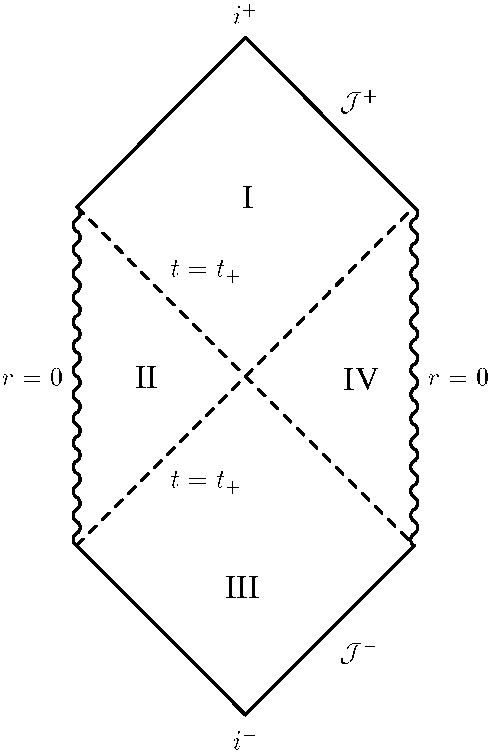
\includegraphics[width=55mm,height=80mm]{Sections/Figures/sbrane.pdf} 
\caption{Penrose diagram for an S-brane. Note that this is a $\pi/2$ rotation of the Schwarzschild black hole Penrose diagram. Regions I and III are cosmological, representing expanding and contracting cosmologies, respectively, separated by smooth horizons which are identified with the S-brane. Regions II and IV are static and have time-like singularities, which can be identified with negative tension end-of-the-world brane-like objects similar to orientifolds. Their corresponding mass and charge can be computed explicitly.} 
\label{sbrane}\end{center}
\end{figure}

More general solutions  of (\ref{einstein}) will have both dilatonic  and  $F_{q+2}$ charges (see for instance \cite{Grojean:2001pv,Burgess:2002vu}). 
The static region provides us with a way to  identify 
this geometry correctly. It turns out that the singularities are the
 physical objects  to which mass, or tension and charge can be
 assigned unambiguously.
It was found that the two singularities correspond to negative tension 
objects, like end-of-the-world branes with opposite charge. 
Furthermore, the similarity with black
hole geometry 
indicates that there will be particle production 
 and we 
 can also compute a generalised Hawking temperature and entropy which could have 
interesting cosmological interpretations. Finally, just as in the case of the Pre Big-Bang, ekpyrotic/cyclic and brane gas scenarios, S-branes naturally have a period of contraction of the universe corresponding to region III of the Penrose diagram, followed by another period of expansion (region I). For further details on the cosmological interpretations of S-branes see for instance \cite{Grojean:2001pv,Burgess:2002vu,Cornalba:2002nv,Cornalba:2002fi,Burgess:2003tz,Kounnas:2011gz,Townsend:2003fx,Ohta:2003pu}.




\subsection{Swampland Conjectures}
\label{Sec:Swamp}

\begin{figure}[t]
\begin{center}
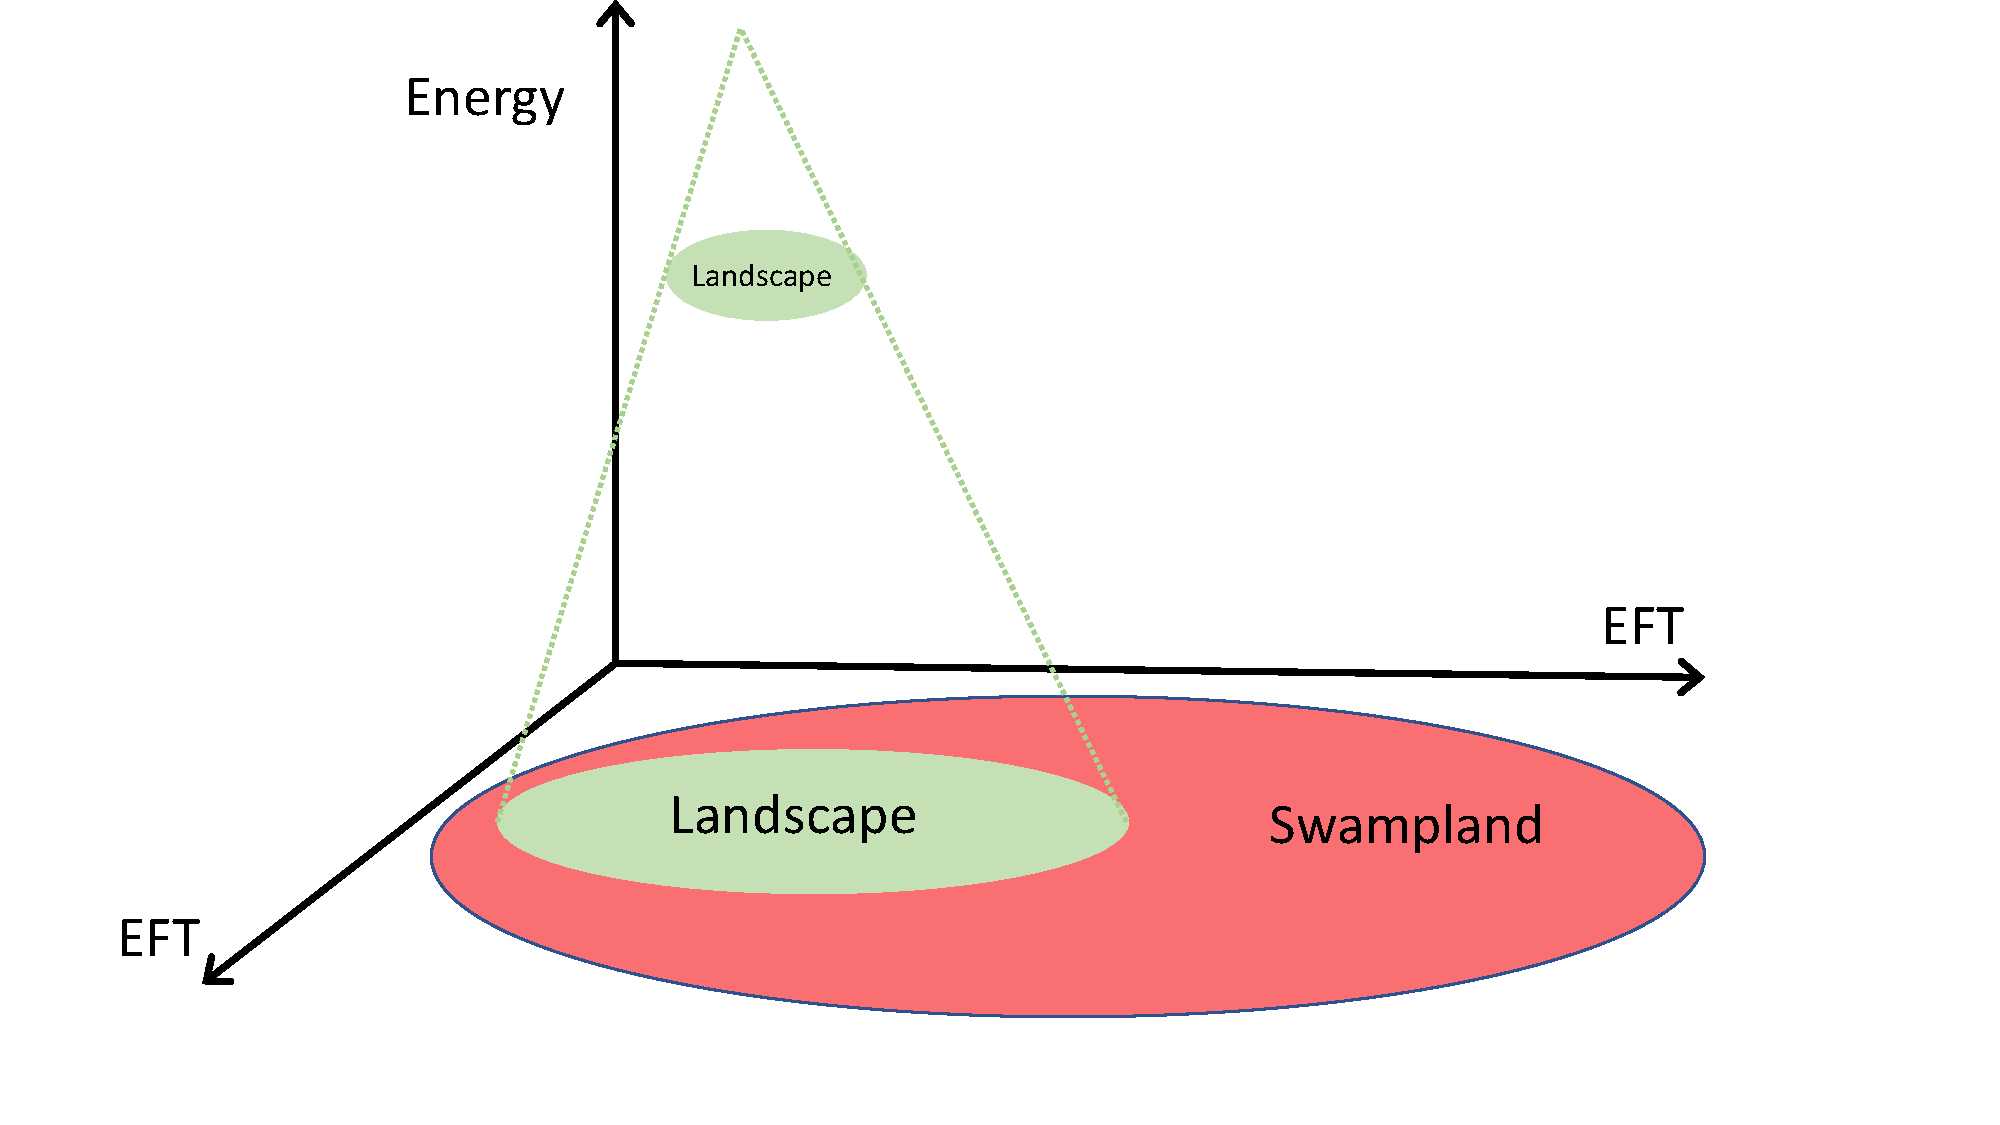
\includegraphics[width=140mm,height=90mm]{Sections/Figures/Swampland.pdf} 
\caption{A cartoon representation of the swampland. At low energies there are many consistent effective field theories, but only a subset of them can be lifted to be UV complete inside a quantum gravity theory. These correspond to the landscape. The rest  are referred to as the swampland.} \label{swampland}
\end{center}
\end{figure}

The vast number of apparent string vacua has very interesting implications. As described in Chapter \ref{sec:DE}, it may be the only self-consistent way to explain the smallness of the dark energy and may provide a totally different approach to asking fundamental questions in physics, separating the `interesting questions' (those that do need an explanation from an underlying theory) from the `uninteresting questions' (those that may be explained by the presence of the multiverse). However, this may also lead to the belief that any theory at all may be derivable from string theory, resulting in a conclusion that it is impossible ever to test string theory, even in principle. This gives the idea of the swampland, illustrated in figure \ref{swampland}.

That said, since the early days of string theory we have known that this is not true: there are some, albeit only a few, general physics properties that can be extracted from string theory. Namely,
\begin{itemize}
\item The need for supersymmetry at the fundamental level (although the scale of its breaking is not known and it may take non-standard forms as in misaligned supersymmetry \cite{Dienes:1994np});
\item
 The existence of extra dimensions, and more concretely only 6 or 7 extra dimensions; 
 \item 
 The existence of moduli fields with specific properties, in particular gravitational-strength couplings, 
 which appear in very specific ways within the low-energy effective field theory; 
 \item The absence of an infinite number of continuous spin representations corresponding to massless particles. These are in principle allowed by the principles of quantum mechanics but have not been observed in nature, despite the lack of alternative explanations from basic principles;
 \item The general absence of global symmetries in the effective field theory.
\end{itemize}

These general results can be complemented with general properties of the landscape, for instance, if the landscape is dominated by Coleman-de Luccia vacuum transitions, a general claim exists that the curvature of the Universe has to be negative, implying an open universe. However, the power of such general results is limited and they still allow for the existence of the enormous landscape resulting in limited predictive power.

In the past few years a new approach towards addressing concrete questions from string theory has been developed and comes under the name of {\it swampland conjectures} \cite{Vafa:2005ui}. The idea is very simple: exploit our cumulative experience of string vacua to extract results that may actually be general. This program aims to state concrete conjectures whose validity may be tested through further exploration of string solutions, either to confirm or rule out the conjecture. The overall goal of the swampland conjectures is:

\begin{quotation}
\emph{Identify which effective field theories are consistent at low energies but cannot be consistent in a UV completion of the theory including gravity.}
\end{quotation}

This is a modern version of what used to be known as {\it vacuum cleaning} in the sense of having a systematic procedure to separate the proper vacua from those that cannot be UV completed. Such conjectures can be made much sharper by going beyond string theory and claiming that the corresponding conjectures will hold for {\it any} theory of quantum gravity, string theory or otherwise. In this sense, string theory is used only to identify the corresponding conjectures, while the swampland approach aims not only to select string vacua, but to identify general properties of any theory of gravity.


More generally, the study of UV constraints on IR physics is a  blooming field that has seen many new conceptual and technical developments recently.
While the swampland programme is one of these developments,  it is worth mentioning a powerful approach, which simply assumes  unitarity, locality, causality, and Lorentz invariance of the, otherwise unknown, UV completion to derive  constraints on the effective field theories, (see \cite{deRham:2022hpx} for a recent overview on these ideas). Combining these approaches may bring the swampland programme to a firmer footing, for example via positivity bounds or bootstrap arguments. 

Over the years, a range of swampland conjectures have been put forward. They range between those that are strongly motivated, but with limited phenomenological or cosmological impact, to conjectures that may have a major impact, but which lack a robust basis and may be considered extremely speculative. There are several excellent reviews on this field in which a detailed discussion of the conjectures has been explained and argued in much detail \cite{Brennan:2017rbf,Palti:2019pca,vanBeest:2021lhn, Grana:2021zvf} to which we refer the reader for further details and the majority of the original references. Here we content ourselves by briefly mentioning those conjectures that could be more relevant for cosmology:

\begin{enumerate}
\item{\it Absence of global symmetries}. A consistent theory of gravity with finite number of states cannot have exact global symmetries. General arguments in this direction have existed since the 1980s: both through arguments that -- contrary to local symmetries -- global symmetries are not protected by black holes after radiation, and also that within string theory, a conformal field theory that leads to a global symmetry also leads to a massless particle in the spectrum that corresponds to the gauge field of that symmetry and therefore the symmetry is not global but local in spacetime \cite{Banks:1988yz}.  More recently, further evidence has accumulated to support its validity. While the general impact of this result is strong, it provides only weak constraints on local symmetries with very weak couplings that to most practical particle physics purposes behave as global symmetries (see for instance \cite{Burgess:2008ri}).

\item {\it Weak gravity conjecture \cite{Arkani-Hamed:2006emk}}. The observational fact that we observe gravity to be the weakest force may not be a property only of our Universe but also of any possible universe described by a consistent theory of gravity. A concrete statement of this conjecture is that in any consistent theory of gravity, there should exist a particle of charge $Q$ and mass $M$ such that $Q^2>GM^2$ (for which the Coulomb force is stronger than the Newtonian force) although more precise and generalised formulations have been proposed \cite{Harlow:2022gzl}. This is the prime example of a  swampland conjecture  that has been argued and tested in sufficiently many ways that there exists a broad consensus that it is actually a correct statement. This has played a useful role in cosmology, especially when extended to forces mediated by scalar fields and  antisymmetric tensors, and in particular when they are dual to axion-like-particles. The weak gravity conjecture may also then be used to constrain the axion decay constant that plays a role in some models of inflation.

\item{\it Cobordism conjecture \cite{McNamara:2019rup}.} Two manifolds are called cobordant if their union is the boundary of another manifold of one extra dimension. This defines an equivalence relation. The corresponding equivalent classes may define a global (topological) charge. We may generalise the absence of global charges conjecture to this topological case and conjecture that  in  a consistent theory of gravity, all cobordism classes have to be trivial. If the corresponding manifolds are, for instance, the 6-dimensional compact spaces, the corresponding 4-dimensional EFTs would be separated by a domain wall (see figure (\ref{cobordism})). If the cobordism class is trivial then it must admit  an end-of-the-world configuration as in the Horava-Witten or bubble of nothing cases (see figure (\ref{cobordism2})). If this conjecture holds, it may have very important implications for cosmology due to the presence of the boundary-ending spacetime. For recent developments in this direction see for instance \cite{Angius:2022aeq,Angius:2022mgh}.

\begin{figure}[t]
\begin{center}
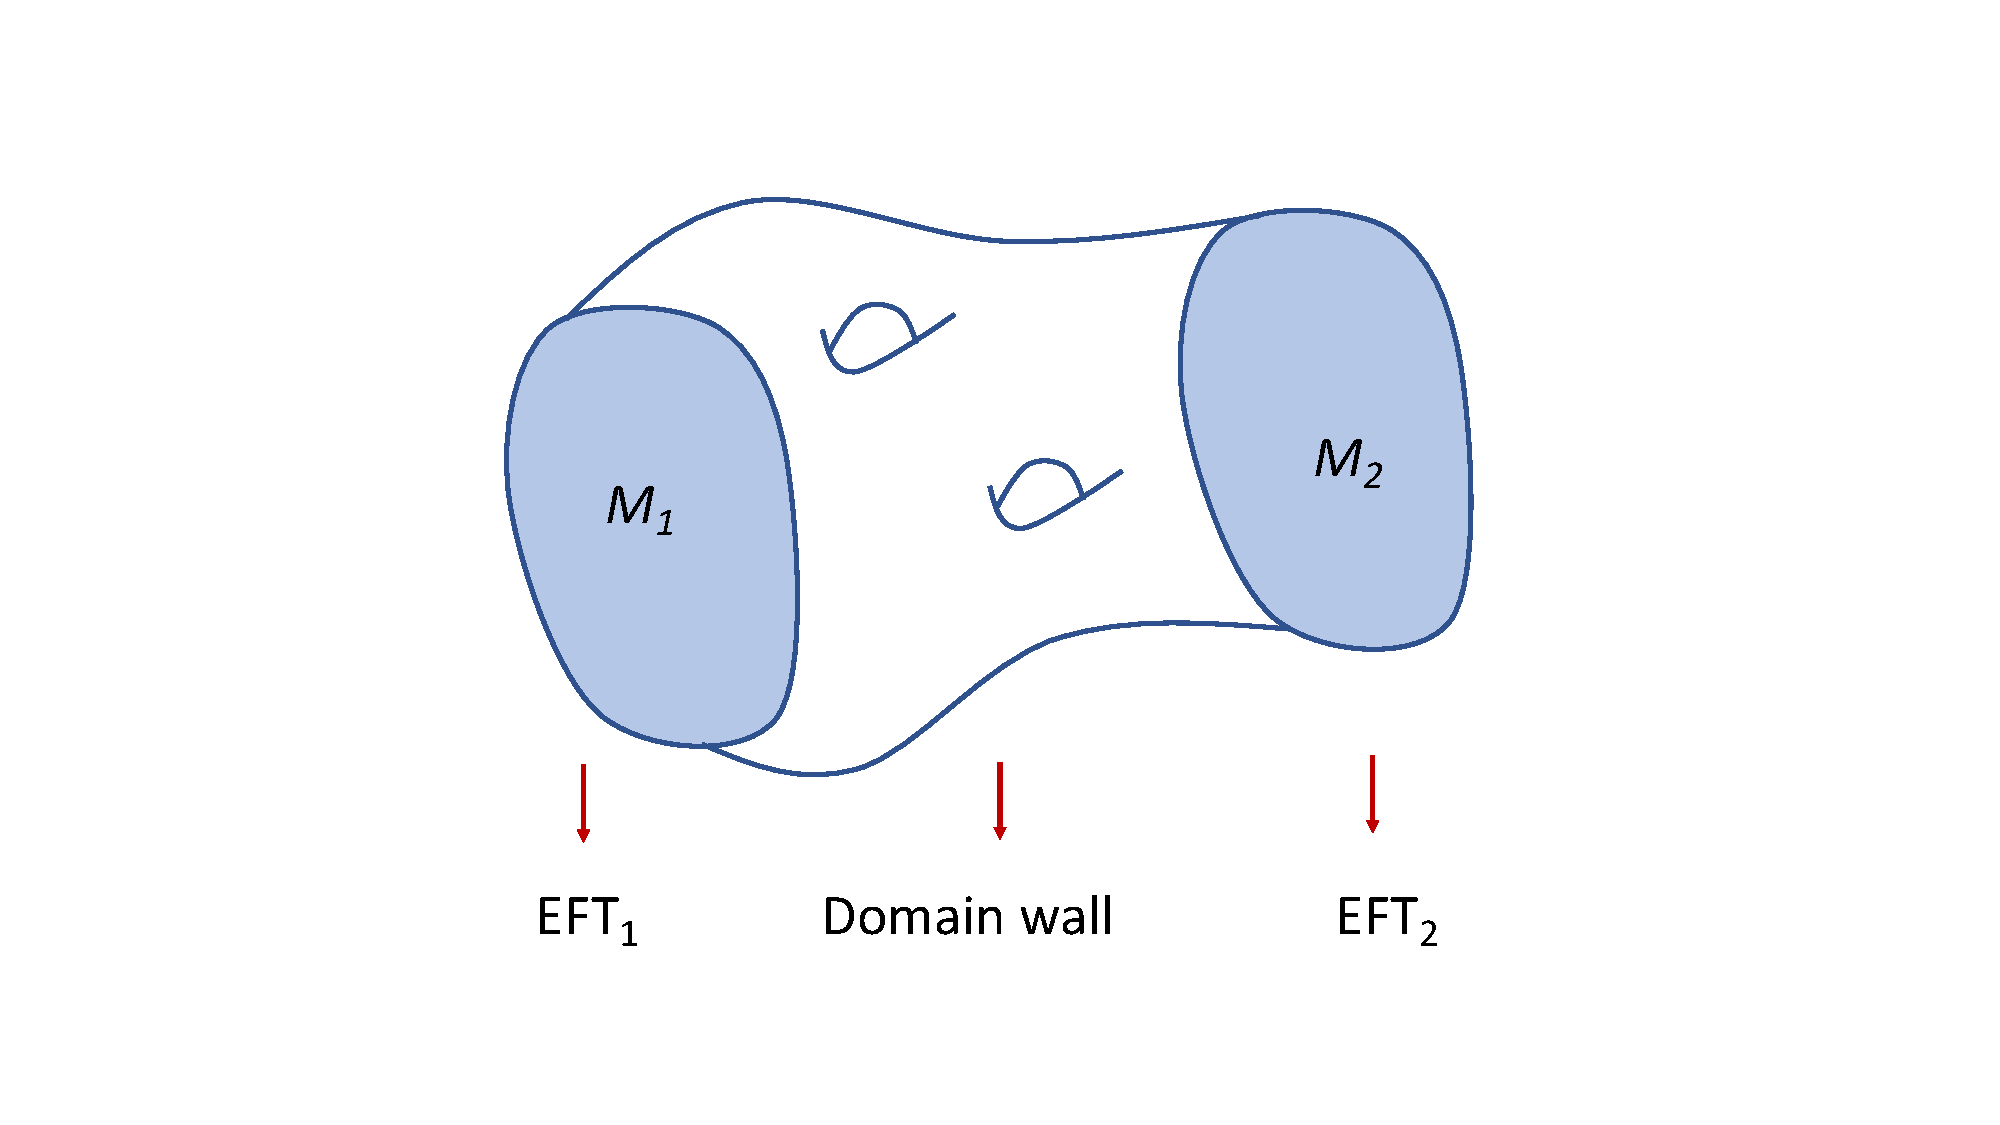
\includegraphics[width=140mm,height=90mm]{Sections/Figures/Cobordism.pdf} 
\vskip -15pt
\caption{A representation of cobordism among two manifolds for which their union is the boundary of another manifold of one extra dimension.} \label{cobordism}
\end{center}
\end{figure}



\item{\it Distance conjecture \cite{Ooguri:2006in}.} 
Consider an effective field theory coupled to gravity with a moduli space, ${\mathcal M}$, parameterised by {\em massless} scalar fields, $\phi_i$, and a metric $\gamma_{ij} (\phi_k)$ which determines the scalar's kinetic terms. 
In standard effective field theories, the consistency and trustworthiness of the dynamics of a scalar field potential $V(\phi)$ is determined by requiring that it does not excite modes with masses above the cutoff, $m \gtrsim \Lambda$.
 As long as this is satisfied, the range of possible values for $\phi$ is not bound by $\Lambda$. The swampland distance conjecture states that this no longer holds if the EFT is consistently uplifted to the UV. 

The swampland distance conjecture states that,  as some modulus approaches a point at infinite {\em geodesic distance} in moduli space, there is an infinite tower of states, which become exponentially massless with the geodesic distance $\Delta\phi$: $m\sim e^{-\Delta\phi}$. These states cannot be neglected from the EFT in this limit. The prime example of such behaviour is when $\phi$ represents the size of an extra dimension and the corresponding tower of states are either the Kaluza-Klein or the winding modes.

As well as infinite limits, the revised distance conjecture also states that for finite displacements, starting from a value $\phi_0$, at a point $\phi_0+\Delta \phi$ infinite towers of modes with mass of order $e^{-\Delta\phi}$ become lighter and lighter with the distance in field space $\Delta\phi$ and so can no longer be neglected from the EFT. Although the conjecture applies to massless scalar fields moving along geodesic trajectories, it could in principle have implications for the field range in single field inflationary models and/or the amount of non-geodesicity in multifield models. However, further work in this direction is needed to establish these possible constraints (see e.g. \cite{Kinney:2018nny, Kinney:2018kew, Palti:2019pca,vanBeest:2021lhn,Grana:2021zvf}).\footnote{ For example, in  \cite{Buratti:2018xjt} it has been shown  that  backgrounds with spacetime varying scalars can  lead to trans-Planckian motion without encountering exponentially falling towers of states. }
 

\begin{figure}[t]
\begin{center}
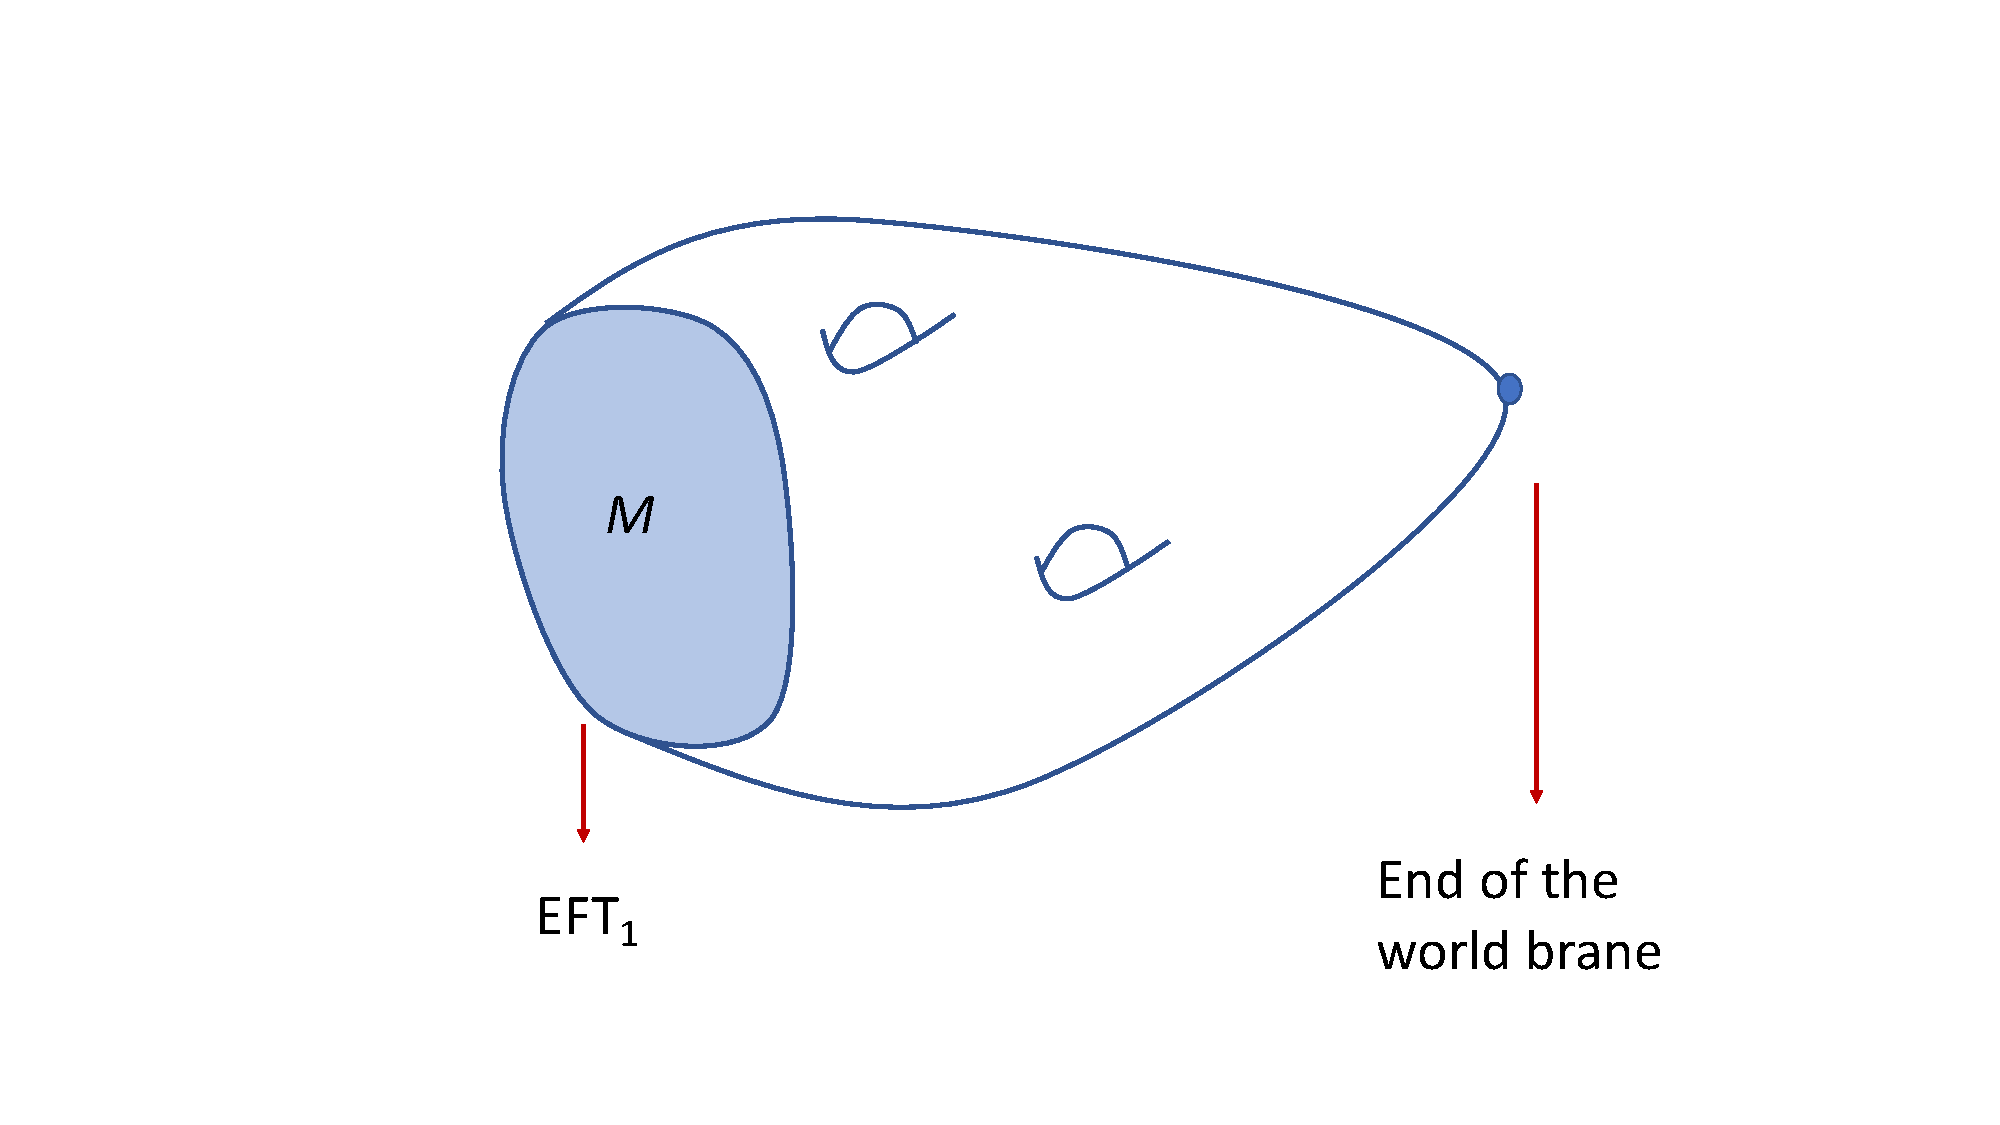
\includegraphics[width=140mm,height=90mm]{Sections/Figures/Cobordism2.pdf} 
\vskip -15pt
\caption{Trivial cobordism with only one manifold in the boundary. The cobordism conjecture states that in this case there should be an end-of-the world configuration.} \label{cobordism2}
\end{center}
\end{figure}


\item{\it Conjectures on  AdS vacua (non-supersymmetric $\&$ supersymmetric):}  Swampland conjectures for non-supersymmetric AdS constructions were proposed in
\cite{Ooguri:2016pdq}. These conjectures are at two levels. The first is motivated by an extension of the weak gravity conjecture; the extension requires that
the equality between electric and gravitational forces is saturated  if and only if the underlying theory is supersymmetric and the states
 under consideration are BPS with respect to the supersymmetry. A consequence of this is that non-supersymmetric AdS solutions supported
 by flux\footnote{A d dimensional AdS solution is said to be supported by flux if a d-form flux field strength   space-fills the AdS space.}  are unstable as they can decay by a brane nucleation process which leads to flux depletion (in a process similar
 to that of \cite{Maldacena:1998uz}). The stronger form of the conjecture removes the requirement that the AdS solution is supported by
 flux and states that  there are no non-supersymmetric AdS solutions in a consistent quantum theory with low energy description in terms of Einstein gravity coupled to a finite number of matter fields. If correct, there will be important  implication not only for moduli stabilisation
 (the AdS vacuum in the LVS scenario is non-supersymmetric) but also for applications of the AdS/CFT correspondence to condensed matter physics, quantum information and hadron physics since the holographic models used in this context have no supersymmetry.  At present, the stronger form of the conjecture does not have much support (see \cite{Baykara:2022cwj} for good evidence in favour of non-supersymmetric AdS vacua in $O(16) \times O(16)$
 heterotic strings). The conjecture can be reformulated in the language of conformal field theories. Conformal field theories dual to Einstein gravity with a finite number of matter fields must satisfy the following (energy) gap condition: they  can have  only a small number of primary fields whose operator products generate all primary fields up to a  energy scale that can be  made parametrically large in the large N limit. The conjecture implies that this condition cannot be met in non-supersymmetric conformal field theories. For attempts to construct such non-supersymmetric conformal field theories meeting this condition see e.g. \cite{Giombi:2017mxl, Gurucharan:2014cva}. 
 
For the relationship of these conjectures of other swampland conjectures, see e.g. \cite{Bernardo:2021vfw}. More recently, it has be put forward that  some  supersymmetric AdS  vacua such as the KKLT AdS solution and pure supergravity AdS lie in the swampland \cite{Lust:2022lfc, Montero:2022ghl}.




\item{\it de Sitter conjecture \cite{Obied:2018sgi}.} It is well known that in string theory both AdS and Minkowski spaces are naturally obtained (mostly because they preserve supersymmetry), while de Sitter space is far more difficult to obtain: a fact which is very important for describing the current acceleration of the Universe through the $\Lambda CDM$ model in terms of the string landscape and early universe inflation. 

The concrete scenarios, such as KKLT and LVS presented in previous sections, provide realisations of de Sitter space from string theory. However, their validity relies on the EFT analysis of perturbative and non-perturbative corrections. As we discussed, the Dine-Seiberg problem that implies the runaway behaviour of the scalar potential for both the volume of the extra dimensions and the dilaton, suggests that in the regime where both perturbative expansions, $g_s$ and $\alpha'$, are under {\it full control}, we should be in the asymptotic runaway region, and so de Sitter vacua at any finite value of the volume or at any non-zero string coupling are in a regime where the approximations cannot be fully trustable. This has led to a bold conjecture stating that there are not actually any de Sitter vacua in a consistent theory of gravity and that the de Sitter vacua found in the literature are only artifacts of the fact that the approximations used are not under full control.\footnote{See also \cite{Cribiori:2020use} for an argument against trustable 4-dimensional dS solutions in $\mathcal{N}=2$ supergravity based on the magnetic weak gravity conjecture.} The original claim was:
\be
\setlength\fboxsep{0.25cm}
\setlength\fboxrule{0.4pt}
\boxed{
|\nabla V|\geq c \frac{V}{\Mp}\,,\qquad 0\leq c \sim {\mathcal{O}}(1)
}
\ee
This condition is clearly satisfied in the Dine-Seiberg runaway regime in which the approximations are under full control. However, the conjecture does not add further information in the weak coupling regions where vacua like KKLT and LVS are claimed to lie. Furthermore, the original conjecture was clearly violated by the Higgs potential (since at the maximum $|\nabla V|=0, V\geq 0$) \cite{Cicoli:2018kdo,Denef:2018etk} (see also \cite{Murayama:2018lie,Choi:2018rze,Hamaguchi:2018vtv}) and a refined version was proposed adding an extra condition on the Hessian of $V$ \cite{Garg:2018reu,Ooguri:2018wrx, Murayama:2018lie}. This conjecture is clearly speculative and less motivated than other swampland conjectures; however, it has motivated further work exploring in more detail  the validity and existence of de Sitter vacua in string theory, which is welcome given the importance of the claim and the challenge.

\item{\it Trans-Planckian censorship conjecture \cite{Bedroya:2019snp,Bedroya:2019tba}.}  It is well known that in inflationary models, microscopic modes redshift due to the expansion of the universe and may become macroscopic and observable at present. If these modes are below the Planck length, it seems to indicate a transfer of modes from the UV to the IR with the UV modes in a regime beyond the validity of the corresponding EFT. The Trans-Planckian censorship conjecture states that in a consistent theory of gravity this UV to IR transfer should not happen, though it does not explain why this should be the case. This puts, for instance, an upper bound on the number of e-folds of inflation. Even though this conjecture has interesting implications for early universe cosmology, the relevance of the constraints on the (time-dependent)  EFT has been questioned in e.g.~\cite{Kaloper:2018zgi,Dvali:2020cgt,Burgess:2020nec,Komissarov:2022gax, Lacombe:2023qfx}.


\end{enumerate}
In summary, the swampland approach brings an interesting perspective to be considered in general discussions of string cosmology. Confirming, discarding or refining these conjectures may lead to relevant progress in the field of string cosmology and, more generally, in principle, to progress in any cosmological implications of consistent theories of quantum gravity. For this much work will be needed.

\subsection{Bubbles of Nothing and the Wave Function of the Universe}

One of the deepest questions a theory of gravity should eventually address is why there is something rather than nothing. This appears a rather philosophical question, as how to define nothingness in a physical theory is unclear. Clearly it is not simply the vacuum state, as we know in 
quantum mechanics the vacuum is not empty. But over the years cosmologists have proposed concrete definitions of nothing (for example, the absence of space, time and matter). The first explicit example was Witten's bubble of nothing (BON) \cite{Witten:1981gj} illustrated in figure \ref{bon}. When considering simple compactifications of five-dimensional Kaluza-Klein theories, he found a transition from the flat five dimensional metric corresponding to a circular fifth dimension of radius $R$: $ds_5^2= ds_4^2+R^2 d\phi^2$, mediated by an instanton with Euclidean metric:
\be
ds^2=\frac{dr^2}{1-R^2/r^2}+r^2\left(d\theta^2+\cos^2\theta d\Omega_2^2 \right)+ \left(1-R^2/r^2\right) R^2 d\phi^2.
\ee
Similar to the Euclidean Schwarzschild metric, this is non-singular even at $r=R$. But this is a minimum value of the coordinate $r$. For large $r$ the metric is asymptotically flat. So this instanton mediates a transition from a flat spacetime with a circle of radius $R$ to a spacetime with maximum value of $r$ where the fifth dimension collapses which we may identify as a {\it bubble of nothing}. The interesting point is that after nucleation the further evolution of the bubble is through expansion at the speed of light, as can be seen by the Wick rotation $\theta\to it$. Since
$\cos\theta \to \cosh t$ the bubble radius increases exponentially with time eating up the full spacetime. In the 5d case, 
this transition depended on the non-existence of supersymmetry and was considered without taking into account moduli stabilisation of the extra dimension. Generalisations to 6d with moduli fixed by fluxes have been found with the similar dramatic outcome \cite{Blanco-Pillado:2010xww,Brown:2011gt}. Furthermore, it was recently argued that these bubbles of nothing are ubiquitous in string compactifications \cite{GarciaEtxebarria:2020xsr} and may represent eventual sources of instabilities (although being non-perturbative, the decay rate may be much suppressed).
\begin{figure}[t]
\begin{center}
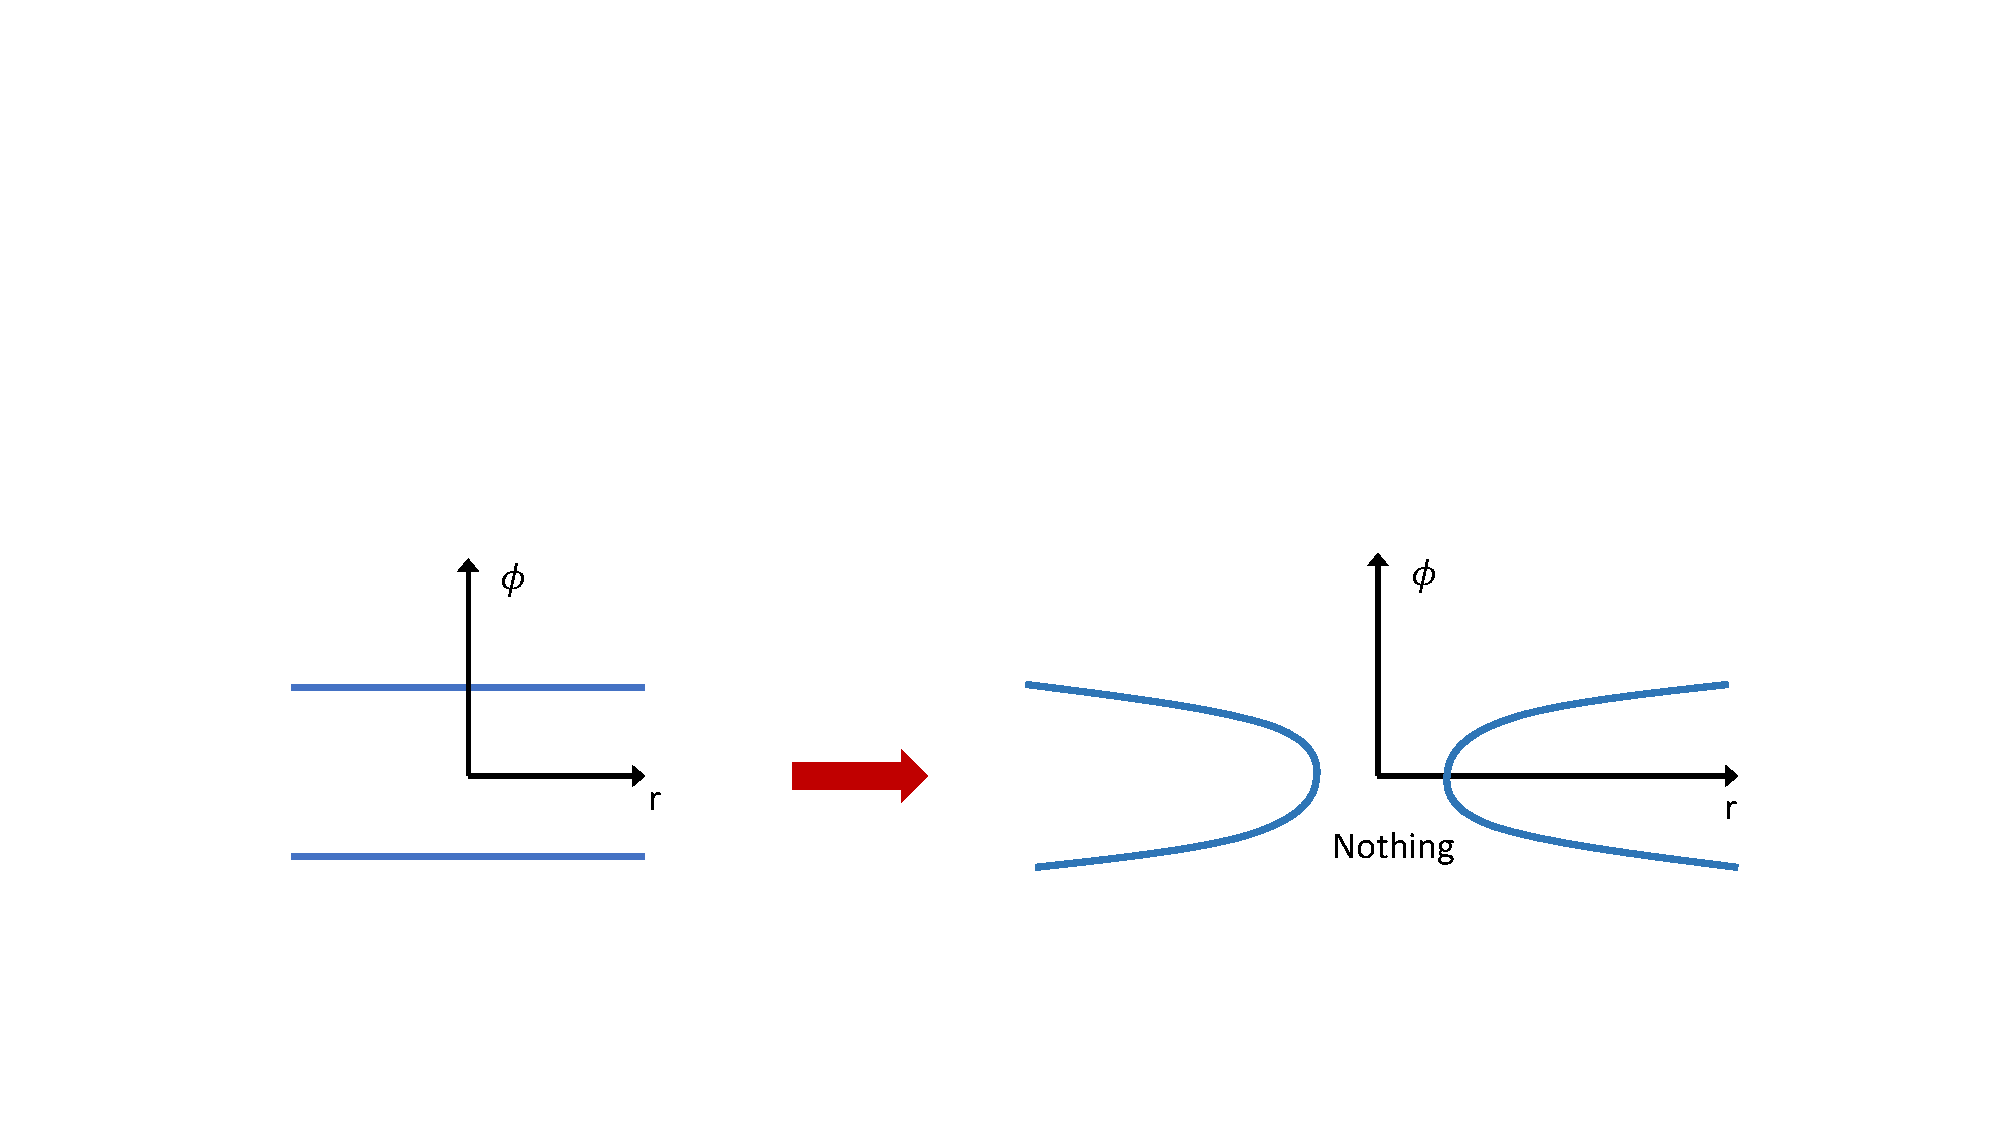
\includegraphics[width=170mm,height=50mm]{Sections/Figures/BON.pdf} 
\caption{An illustration of the Bubble of Nothing scenario: a transition resulting to an expanding absence of space-time. On the left we have the flat 4d in the horizontal  and the extra dimension in the vertical with the two horizontal lines identified in a circle compactification. On the right the transition to the bubble of nothing. For large $r$ it is as in the left but for smaller values of $r$ at some point the extra dimension collapses and a bubble of nothing appears (a cross section is shown) and expands in time.} \label{bon}
\end{center}
\end{figure}

The second appearance of nothing was in the {\it creation out of nothing} scenario of Vilenkin \cite{Vilenkin:1982de,Vilenkin:1983xq,Vilenkin:1984wp} and the subsequent {\it wave function of the universe} of Hartle and Hawking \cite{Hartle:1983ai}. See also\cite{Linde:1983mx,Rubakov:1999qk,Hartle:2022jkt}. This  defines, within the domain of semiclassical gravity, a concrete proposal to describe the beginning of the universe from a state with no spacetime. So, in a sense it is the opposite of the bubble of nothing picture. 

From simple mini-superspace arguments the transition from nothing to a de Sitter space with cosmological constant given by $H^2>0$ is found to be of order 
\be
{\mathcal P}=|\Psi|^2\propto\, e^\frac{\eta\, \pi}{2G_4H^2},
\ee
with $\eta=+1$ for Hartle-Hawking boundary conditions (the no boundary proposal in which the nucleated universe is a superposition of expanding and contracting ones) and $\eta=-1$ for the Vilenkin or tunneling transition (for which the boundary conditions are such that they only give an expanding universe). Note that, up to normalisation factors, the Hartle-Hawking wave function favours smaller values of the cosmological constant, making it hard to justify inflation, whereas the Vilenkin normalisation prefers larger values of $H^2$. All these discussions are only within a simplified picture of mini-superspace and semiclassical gravity and, in principle, need to be further studied, especially once a proper quantum gravity theory is at hand. This has been a challenge for string theory and, despite several attempts, the study of such transitions is still in its infancy.

Note that this approach is similar in spirit to the vacuum transitions initiated by Coleman and de Luccia (CDL) which have been inherited in the discussions of the landscape. However, contrary to CDL transitions, here there is no bubble nucleated but instead a full spacetime. This can be done for de Sitter since it has finite volume but for AdS and Minkowski it may require introducing a cut-off in order to quantify the corresponding probability. Furthermore, contrary to the CDL case in which naturally the transition gives rise to an open universe, here, the de Sitter slicing that gives finite volume corresponds to a closed universe \cite{Hartle:2013oda,Cespedes:2020xpn}. This is important since there have been claims that the main general prediction of the string landscape is that it predicts open universes \cite{Freivogel:2005vv,Kleban:2012ph} and if eventually, in the maybe long future, open universes would be ruled out it could  be a strong argument against the landscape. But if closed universes can be created from nothing, settling the curvature of the universe may only differentiate between the two mechanisms. Clearly further studies in these directions are needed.\footnote{An important direction is
bubble stability, see e.g \cite{Johnson:2019tgc} for a recent analysis.} For string theoretical discussions of the wave function of the universe see for instance \cite{Ooguri:2005vr,Brustein:2005yn}.

\subsection{Holography and Cosmology}

The main theoretical development in string theory over the past 25 years has been holography. A gravitational theory in $d$ dimensions is equivalent to a non-gravitational theory in $(d-1)$-dimensions. One old motivation for this equivalence is the well known fact that the black hole entropy, being an extensive quantity, is proportional to the area of its horizon rather than to the internal volume of the black hole. 
The AdS/CFT correspondence now represents the best concrete definition of quantum gravity in anti-de Sitter space (AdS) since, at least in principle, the non-gravitational conformal field theory (CFT) on the boundary of AdS is understood, and any quantum aspects of the gravitational theory can be referred to concrete questions on the CFT side.

Although technically AdS/CFT remains a conjecture,
the evidence for the correspondence is by now overwhelming. In particular, this correspondence has provided a framework which 
allows the black hole loss of information puzzle stated by Hawking almost 50 years ago to be addressed. Holography 
 indicates that, as the CFT side is a standard quantum system, information cannot be lost. Therefore, if the equivalence is correct, 
information also cannot be lost within the gravitational system. Furthermore, using holographic arguments it has also recently been possible to calculate explicitly the entanglement entropy of black holes showing the Page curve behaviour that would be 
expected if the information is not lost\footnote{For studies of implication of entanglement (in particular Bell inequalities) in the cosmological context see \cite{Maldacena:2015bha, Choudhury:2016cso}.}.

It is therefore very appealing to try to extract cosmological implications of holography. Even though our universe is not of the AdS type, several approaches have been proposed, aiming to extend the success of AdS/CFT to cosmological questions. The general topic of holography is so vast 
that we will touch on it even more briefly than for previous subjects and refer the reader to the literature for more details. For recent reviews see for instance \cite{Anninos:2012qw, Flauger:2022hie}.

\begin{enumerate}
\item {\it AdS/CFT  and density perturbations in inflation.} 

One possibility to use AdS/CFT for inflation is to consider a simple potential with two minima with opposite signs of the cosmological constant. 
One minimum corresponds to a stable AdS vacuum and the other to a nearby metastable dS vacuum. The bulk geometry 
near the AdS vacuum is described by boundary CFT and so this can be used to extract information about bubbles of the dS phase from the CFT spectrum \cite{Freivogel:2005qh} (see however \cite{DeAlwis:2019rxg}) and, through analytic continuation, connect the correlators from AdS/CFT to a potential dS/CFT .

In a different direction, assuming that inflationary cosmology has a CFT dual there have been explicit efforts to quantify this 
relation by computing density perturbations using a QFT dual. In particular, known inflationary results regarding
 density perturbations are reproduced in the weak gravity regime. Exploring the domain of strongly coupled gravity by working with 
 the weakly coupled QFT offers an alternative phenomenology to inflation in which an almost scale invariant spectrum of 
 perturbations is also obtained. See e.g. \cite{Freivogel:2005qh, McFadden:2009fg, Bzowski:2012ih, Kundu:2014gxa} for concrete calculations in this
  interesting direction.

\item {\it dS/CFT and dS/dS proposals.} 

A dS/CFT correspondence
 was proposed in \cite{Strominger:2001pn}, following parallels with the
well established AdS/CFT correspondence,
 motivated by the close connection between dS and AdS spaces.
The argument is that a boundary at infinity of, say,  dS$_4$ corresponds to a Euclidean $R_3$
space for which the symmetry group of de Sitter space, $SO(4,1)$ acts as the conformal group
of the Euclidean $R_3$, suggesting that a conformal field theory on this boundary is dual to the full 4D gravity theory in de Sitter space.

 One of the interesting outcomes of
 this conjecture is that the renormalisation group parameter can be identified with
time, in much the same way it was identified with the extra spatial 
coordinate in the AdS/CFT case \cite{Strominger:2001gp}. One simple way to see this possibility is 
by writing the dS$_4$ metric in FRW coordinates ($k=0$) as
\be
ds^2\ = \ -dt^2\ + \ e^{Ht}\ d\vec{x}^{\,\,2},
\ee
with $\vec{x}$ the spatial coordinates 
 and $H$ the Hubble parameter. 
 
 The interesting observation is that this
 metric is invariant under
$t\rightarrow t+\lambda$, $\vec{x}\rightarrow e^{-\lambda H}\vec{x}$ which 
generates time evolution in the 4D bulk and scale transformations on the
 Euclidean boundary.
Late times (large values of $\lambda$) correspond to small distances (UV
 regime) whereas earlier 
times correspond to low energies and the IR regime.
Generic expressions for the scale factor $a(t)$ will not have this symmetry,
but if we assume that
$H(t)$ goes to a constant both in the infinite past and infinite future we can 
follow the time evolution
between two fixed points under the renormalisation group, which could
 eventually be identified
with early universe inflation and also current acceleration. 

The monotonic evolution in time fits well  with the 
expected c-theorem of field theories, holding in 2D, and the extension to the a-theorem in 4d.
The RG flow then corresponds to the direction from future to past. 

As a side note, the S-branes mentioned previously were
 an attempt to bring this correspondence closer to the AdS/CFT one, with the
 S-branes playing the role of the D-branes in the
boundary (the Euclidean $R_3$ in the example above).

A final independent and interesting alternative is the dS/dS correspondence in which a dS space is proposed to be dual to another dS space in one dimension less \cite{Alishahiha:2004md,Dong:2010pm}. This is partly based on the simple observation that the de Sitter dS$_d$ metric in $d$ dimensions can be seen as a warped compactification to dS$_{d-1}$:
\be
ds_d^2=d\omega^2+\sin^2\left(\frac{\omega}{R_{dS}}\right) ds_{d-1}^2.
\ee
Similarly to AdS/CFT, this implies an emergent spatial dimension and warped throats (two in this case since the warp factor vanishes at $\omega=0,\pi R_{dS}$), but contrary to AdS/CFT the dual is no longer a field theory without gravity but now a lower dimensional de Sitter space with a massless graviton.

Even though de Sitter space realisations in string theory are of interest, these potential dS/CFT or dS/dS dualities are not yet under firm grounds, unlike the AdS/CFT case, and much work needs to be done to turn these proposals into something useful for cosmology.

Further proposals for holography and cosmology have been put forward. See for instance \cite{Banks:2003ta}.

\item {\it Islands and cosmology}

A more recent development relates to the progress regarding the information loss paradox in black holes. The main new ingredient here is the concept of quantum extremal surfaces (QES) \cite{Ryu:2006bv,Hubeny:2007xt,Faulkner:2013ana,Engelhardt:2014gca} to generalise the expression for the von Neumann entropy. This prescription gives rise to a time evolution of the entropy such that it increases monotonically up to a maximum point where it starts decreasing, giving rise to what is called a Page curve as required for a unitary evolution  to address the information loss paradox. The key component of this calculation is an entanglement  {\it island} which is a region behind the black hole horizon that hosts the corresponding  degrees of freedom that avoid information loss \cite{Penington:2019npb,Almheiri:2019psf}.

The details of these results are beyond the scope of this review (for a review with all the relevant references see for instance \cite{Almheiri:2020cfm}). However, a notable point is that these results were achieved without the need for a full UV completion of semiclassical gravity. This gives more credibility to semiclassical approaches to quantum cosmology, such as the wave function of the Universe and vacuum transitions discussed above. Furthermore, concepts like quantum extremal surfaces and islands may also play an important role for cosmology. This has been recently explored in 
%
\cite{VanRaamsdonk:2020tlr,Hartman:2020khs,Chen:2020tes,VanRaamsdonk:2021qgv,Geng:2021wcq,Pasquarella:2022ibb, Bousso:2022gth} but it is fair to say that this direction is still in an infancy and there is much to be explored. 

\item{\it Emergence of spacetime}

One point that may be worth pointing out is the recent ideas regarding the emergence of time.  From the original AdS/CFT correspondence, it is clear that not only gravity but also at least one spatial dimension is emergent from the boundary CFT theory (in one less dimension and no gravity). More recent studies of the closed connection between gravitational theories and quantum entanglement have led to the proposals of getting spacetime from entanglement. The proposal of ER=EPR (Einstein-Rosen wormhole equivalent to the Einstein-Podolsky-Rosen entanglement) is a variation of this. Contrary to the emergence of spatial dimensions, the emergence of time has been more challenging to implement. But recent work has been done in this direction. See for instance \cite{Leutheusser:2021frk, Witten:2021unn, Chandrasekaran:2022eqq, Chandrasekaran:2022cip, Leutheusser:2022bgi,Cotler:2023xku}. These subjects fall beyond the scope of the present review and we refer the reader to the papers mentioned and references therein.





\end{enumerate}

Other approaches to string cosmology have been proposed with different levels of development. We would like to note the cosmology of matrix models, which, even though it has not been much explored, matrix models \cite{Banks:1996vh,Ishibashi:1996xs} are one of the few proposals (together with AdS/CFT)  for a non-perturbative formulation of string theory and may deserve further study. We refer to the recent review \cite{Brahma:2022ikl} for the progress and challenges of this approach. 

 \newpage



